\chapter{Examples}
\label{chptr:examples}
This chapter contains some examples of how the Substitution Stepper steps some of the examples from the task description.
The derivations are somewhat long still compared to the examples given in the task description.

\section{Example 1}
The first example sums up three elements in a list.
Due to the limitations of the stepper,
the Nat datatype was used instead of Int.

\begin{figure}
    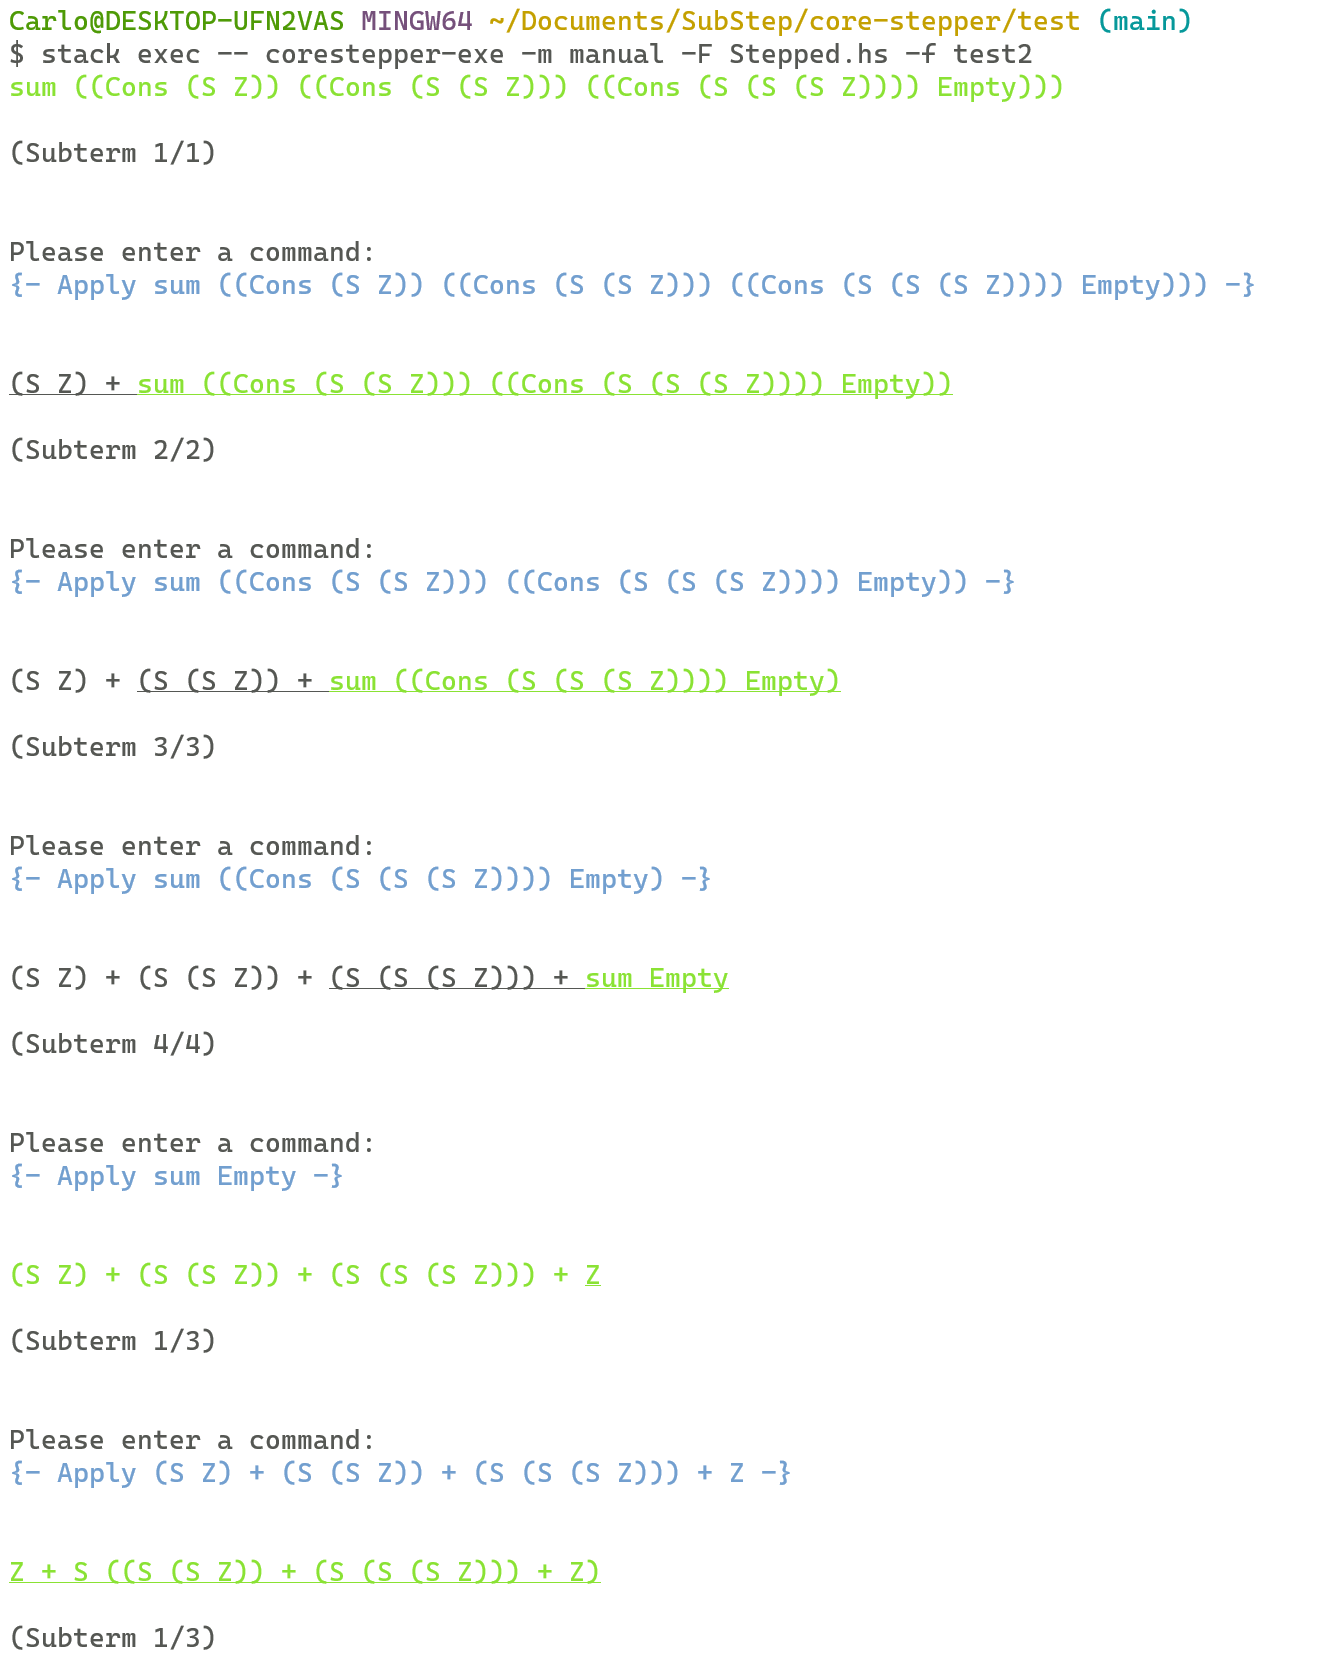
\includegraphics[width=1\textwidth]{resources/sum_part_1.PNG}
\end{figure}
\begin{figure}
    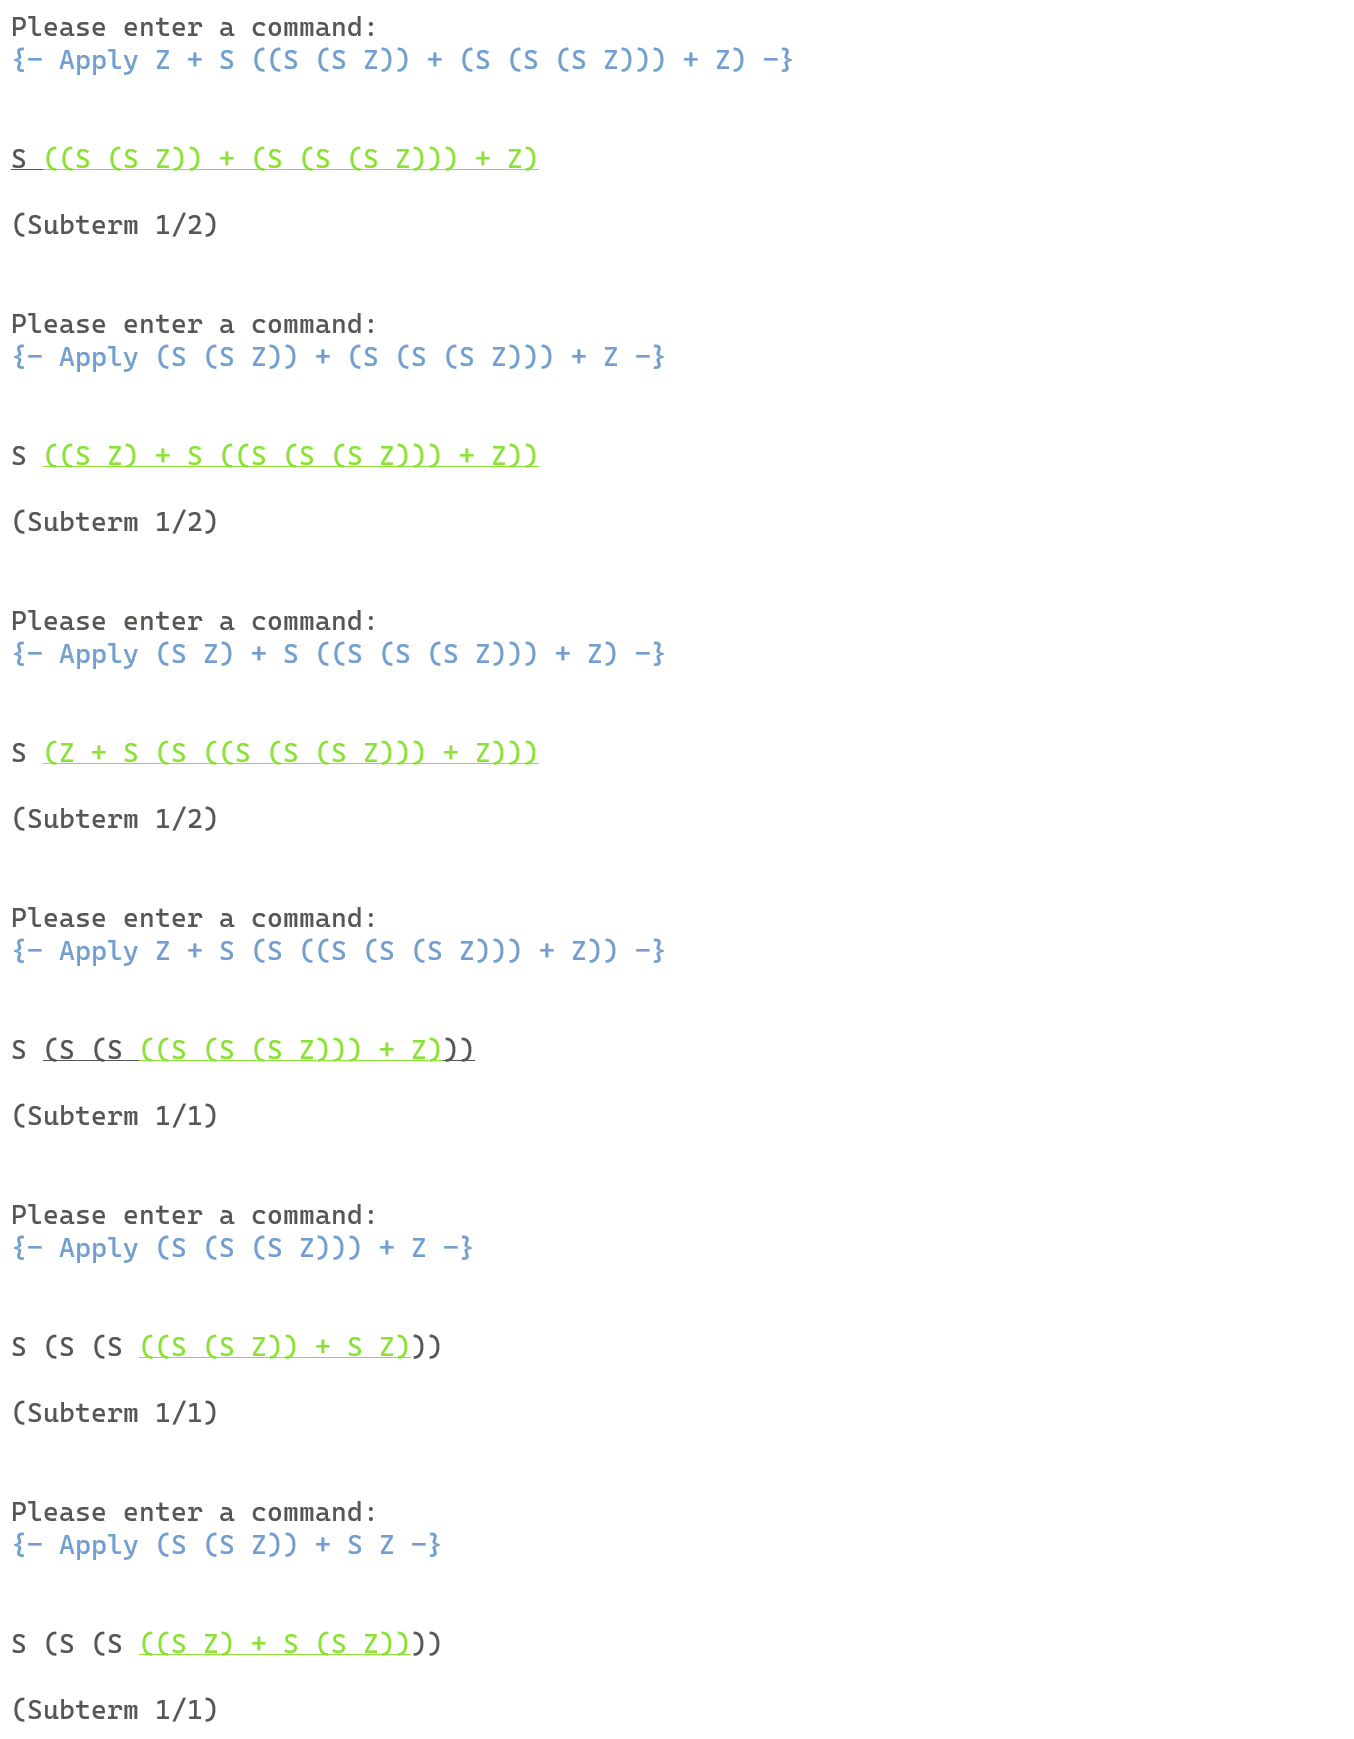
\includegraphics[width=1\textwidth]{resources/sum_part_2.PNG}
\end{figure}
\begin{figure}
    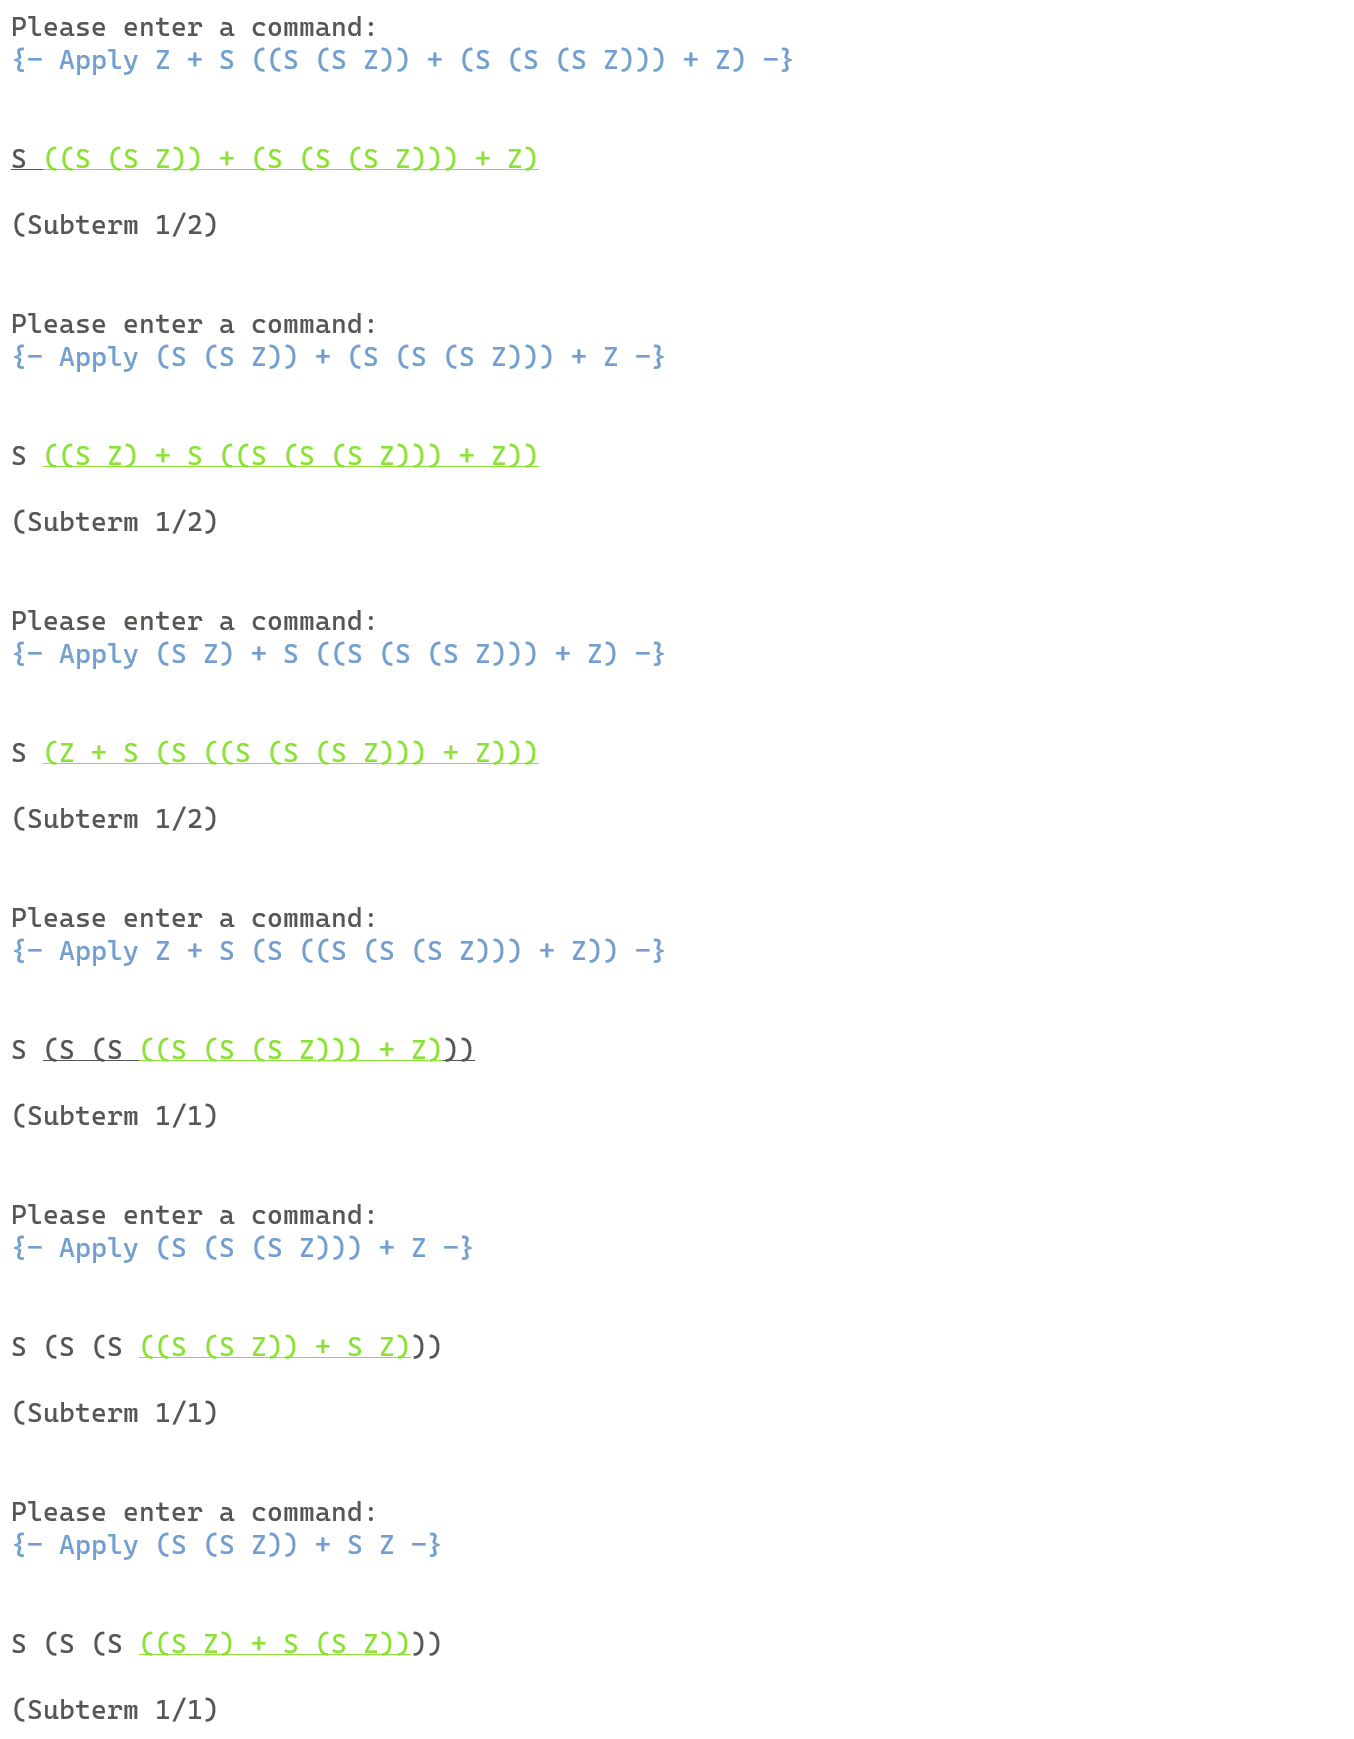
\includegraphics[width=1\textwidth]{resources/sum_part_2.PNG}
    \caption{The first example, summing 1, 2, and 3 in a list to obtain the value 6.}
\end{figure}

\clearpage
\section{Example 2}
The second example reverses a list containing 3 elements.
Again, this example had to be adjusted, this time it uses letters as they are more easily readable than the Nat datatype.

\begin{figure}
    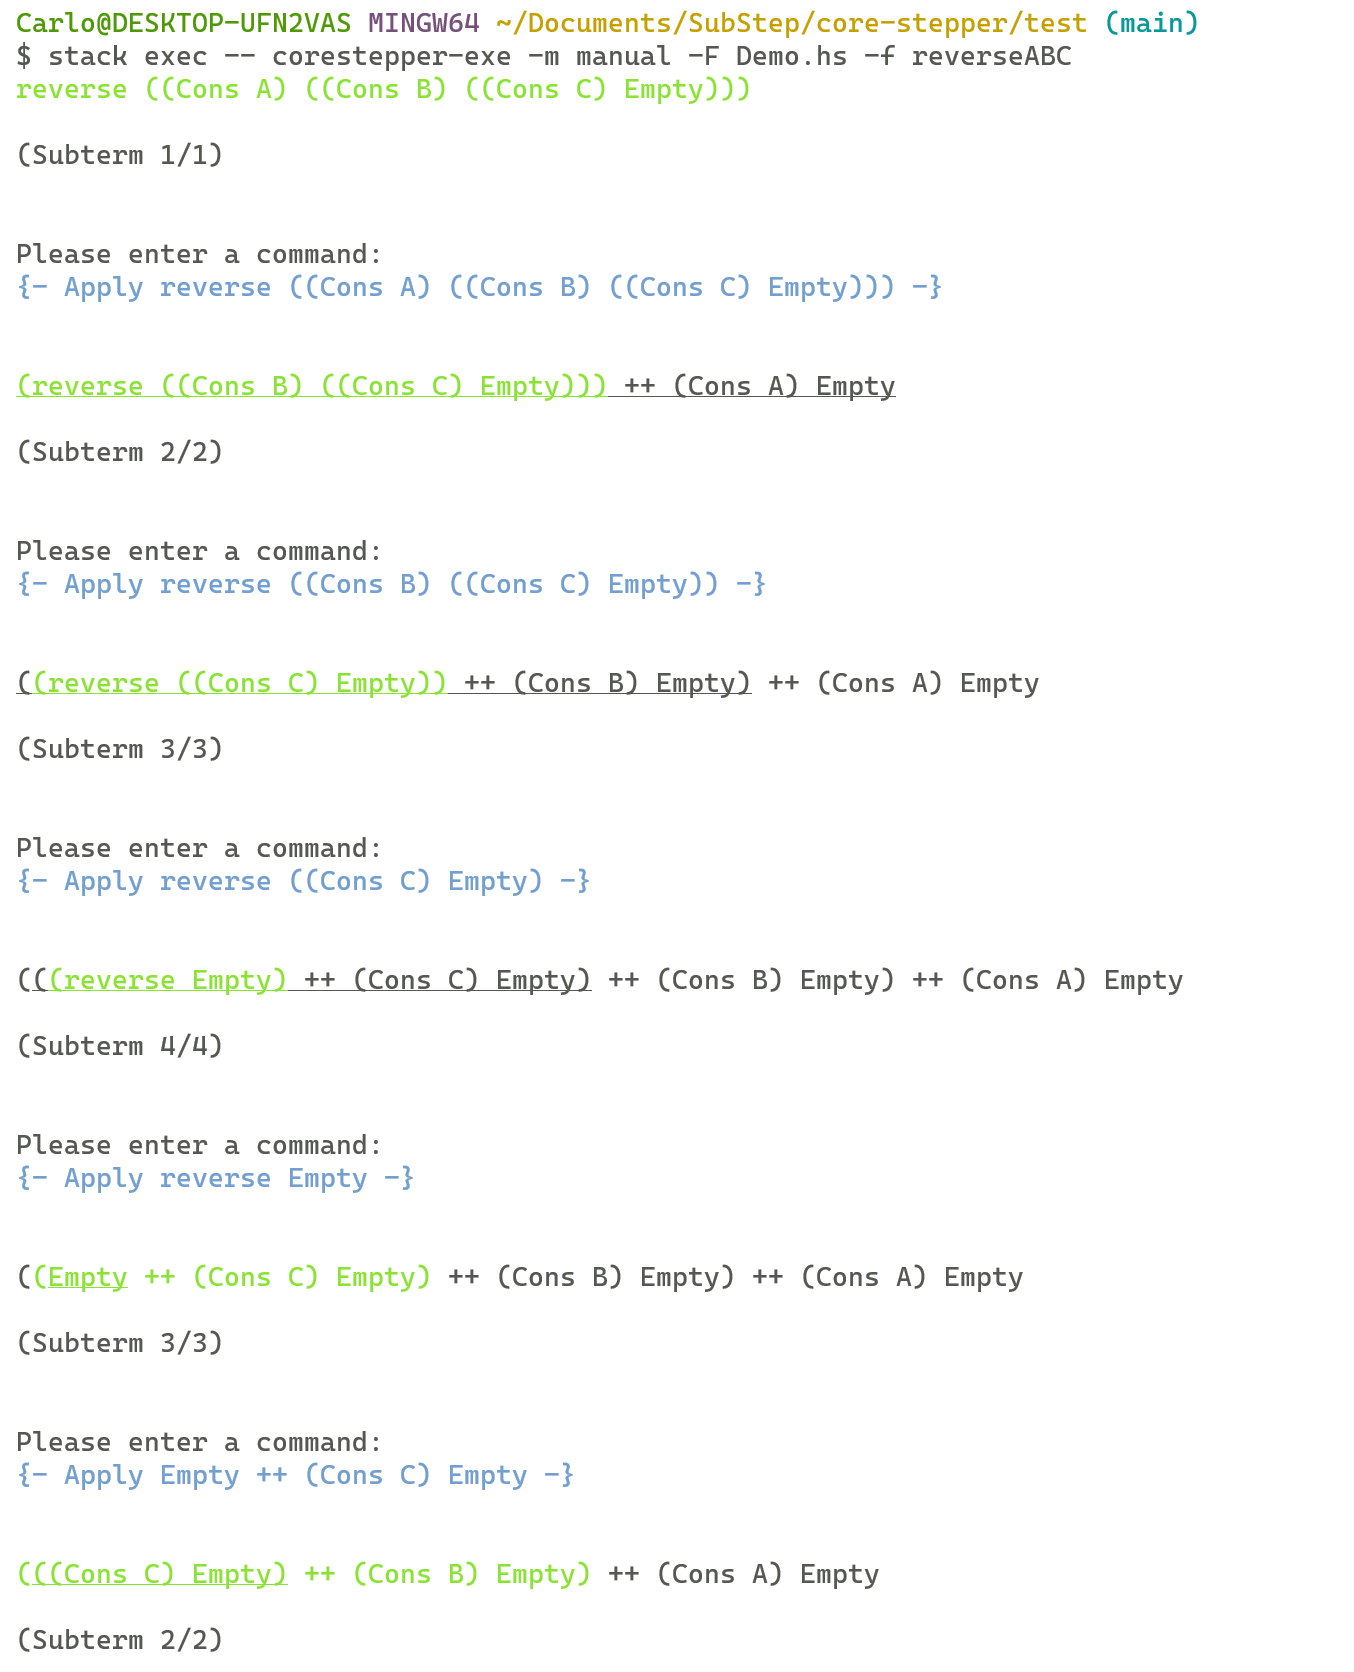
\includegraphics[width=1\textwidth]{resources/reverse_part_1.PNG}
\end{figure}
\begin{figure}
    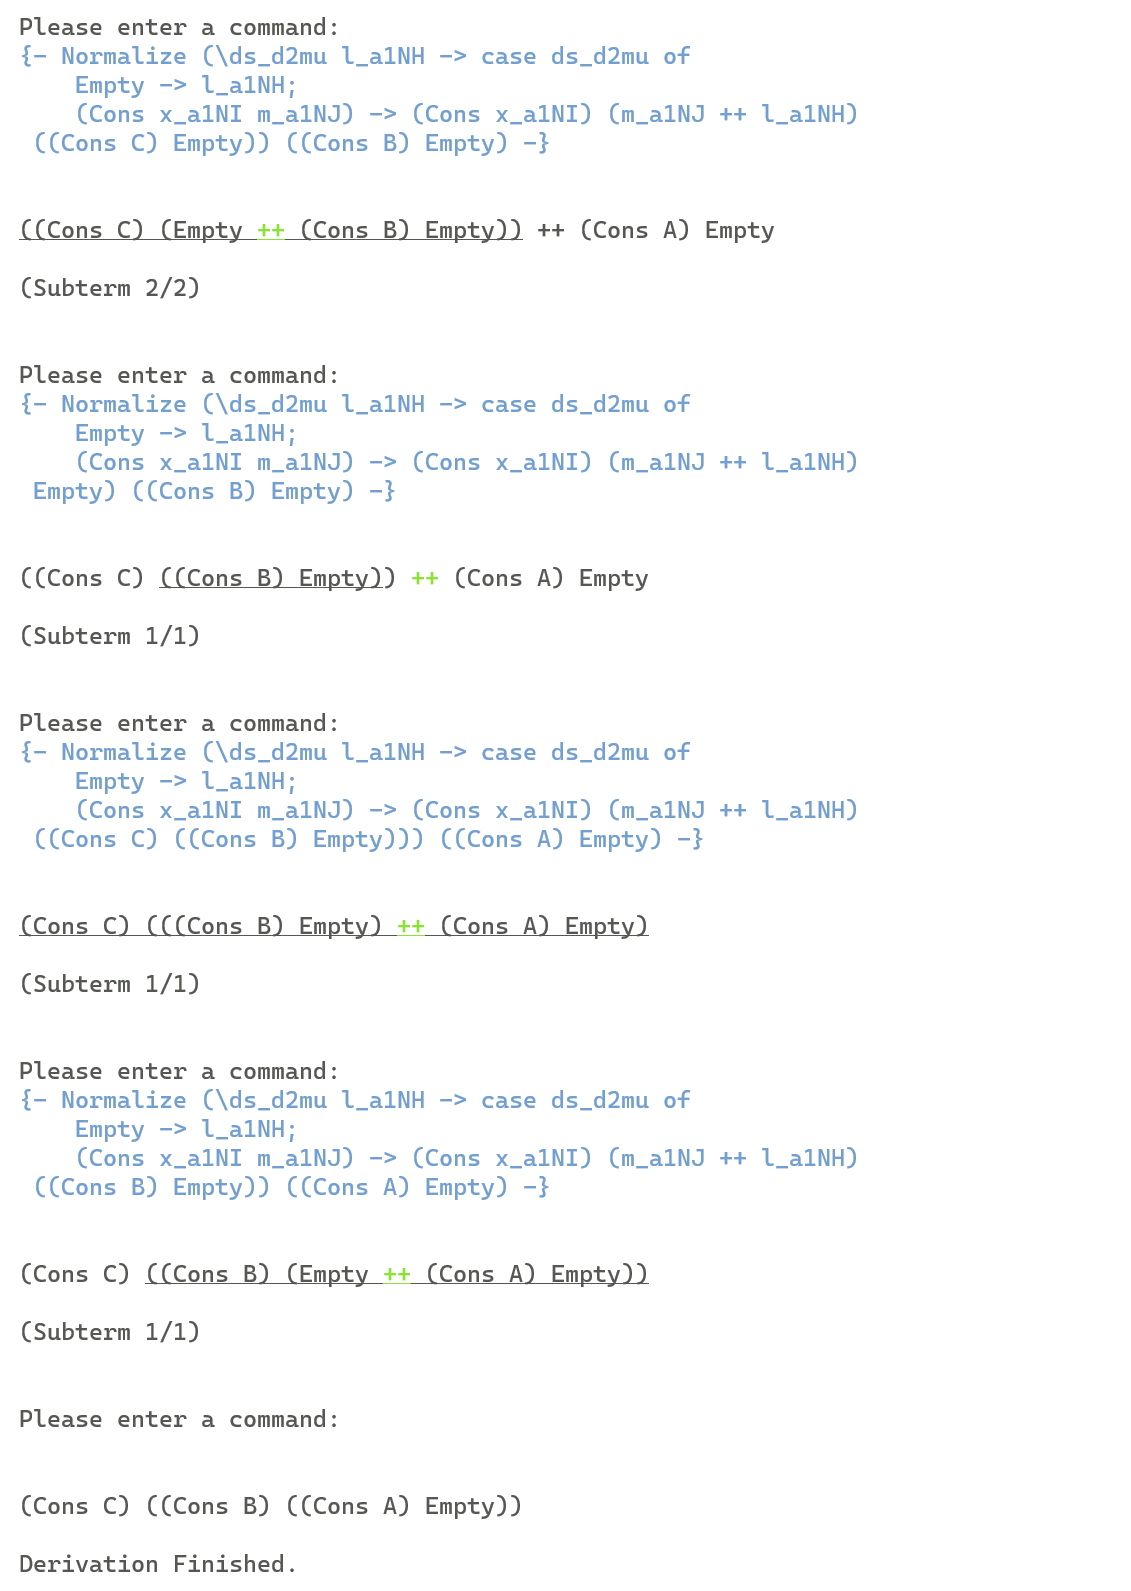
\includegraphics[width=1\textwidth]{resources/reverse_part_2.PNG}
    \caption{The second example, reversing the list [A,B,C].}
\end{figure}

\clearpage
\section{Example 3}
The third example uses the Nat datatype again.
It corresponds to \texttt{pure (+) <*> [1,2] <*> [3,4]}

\begin{figure}
    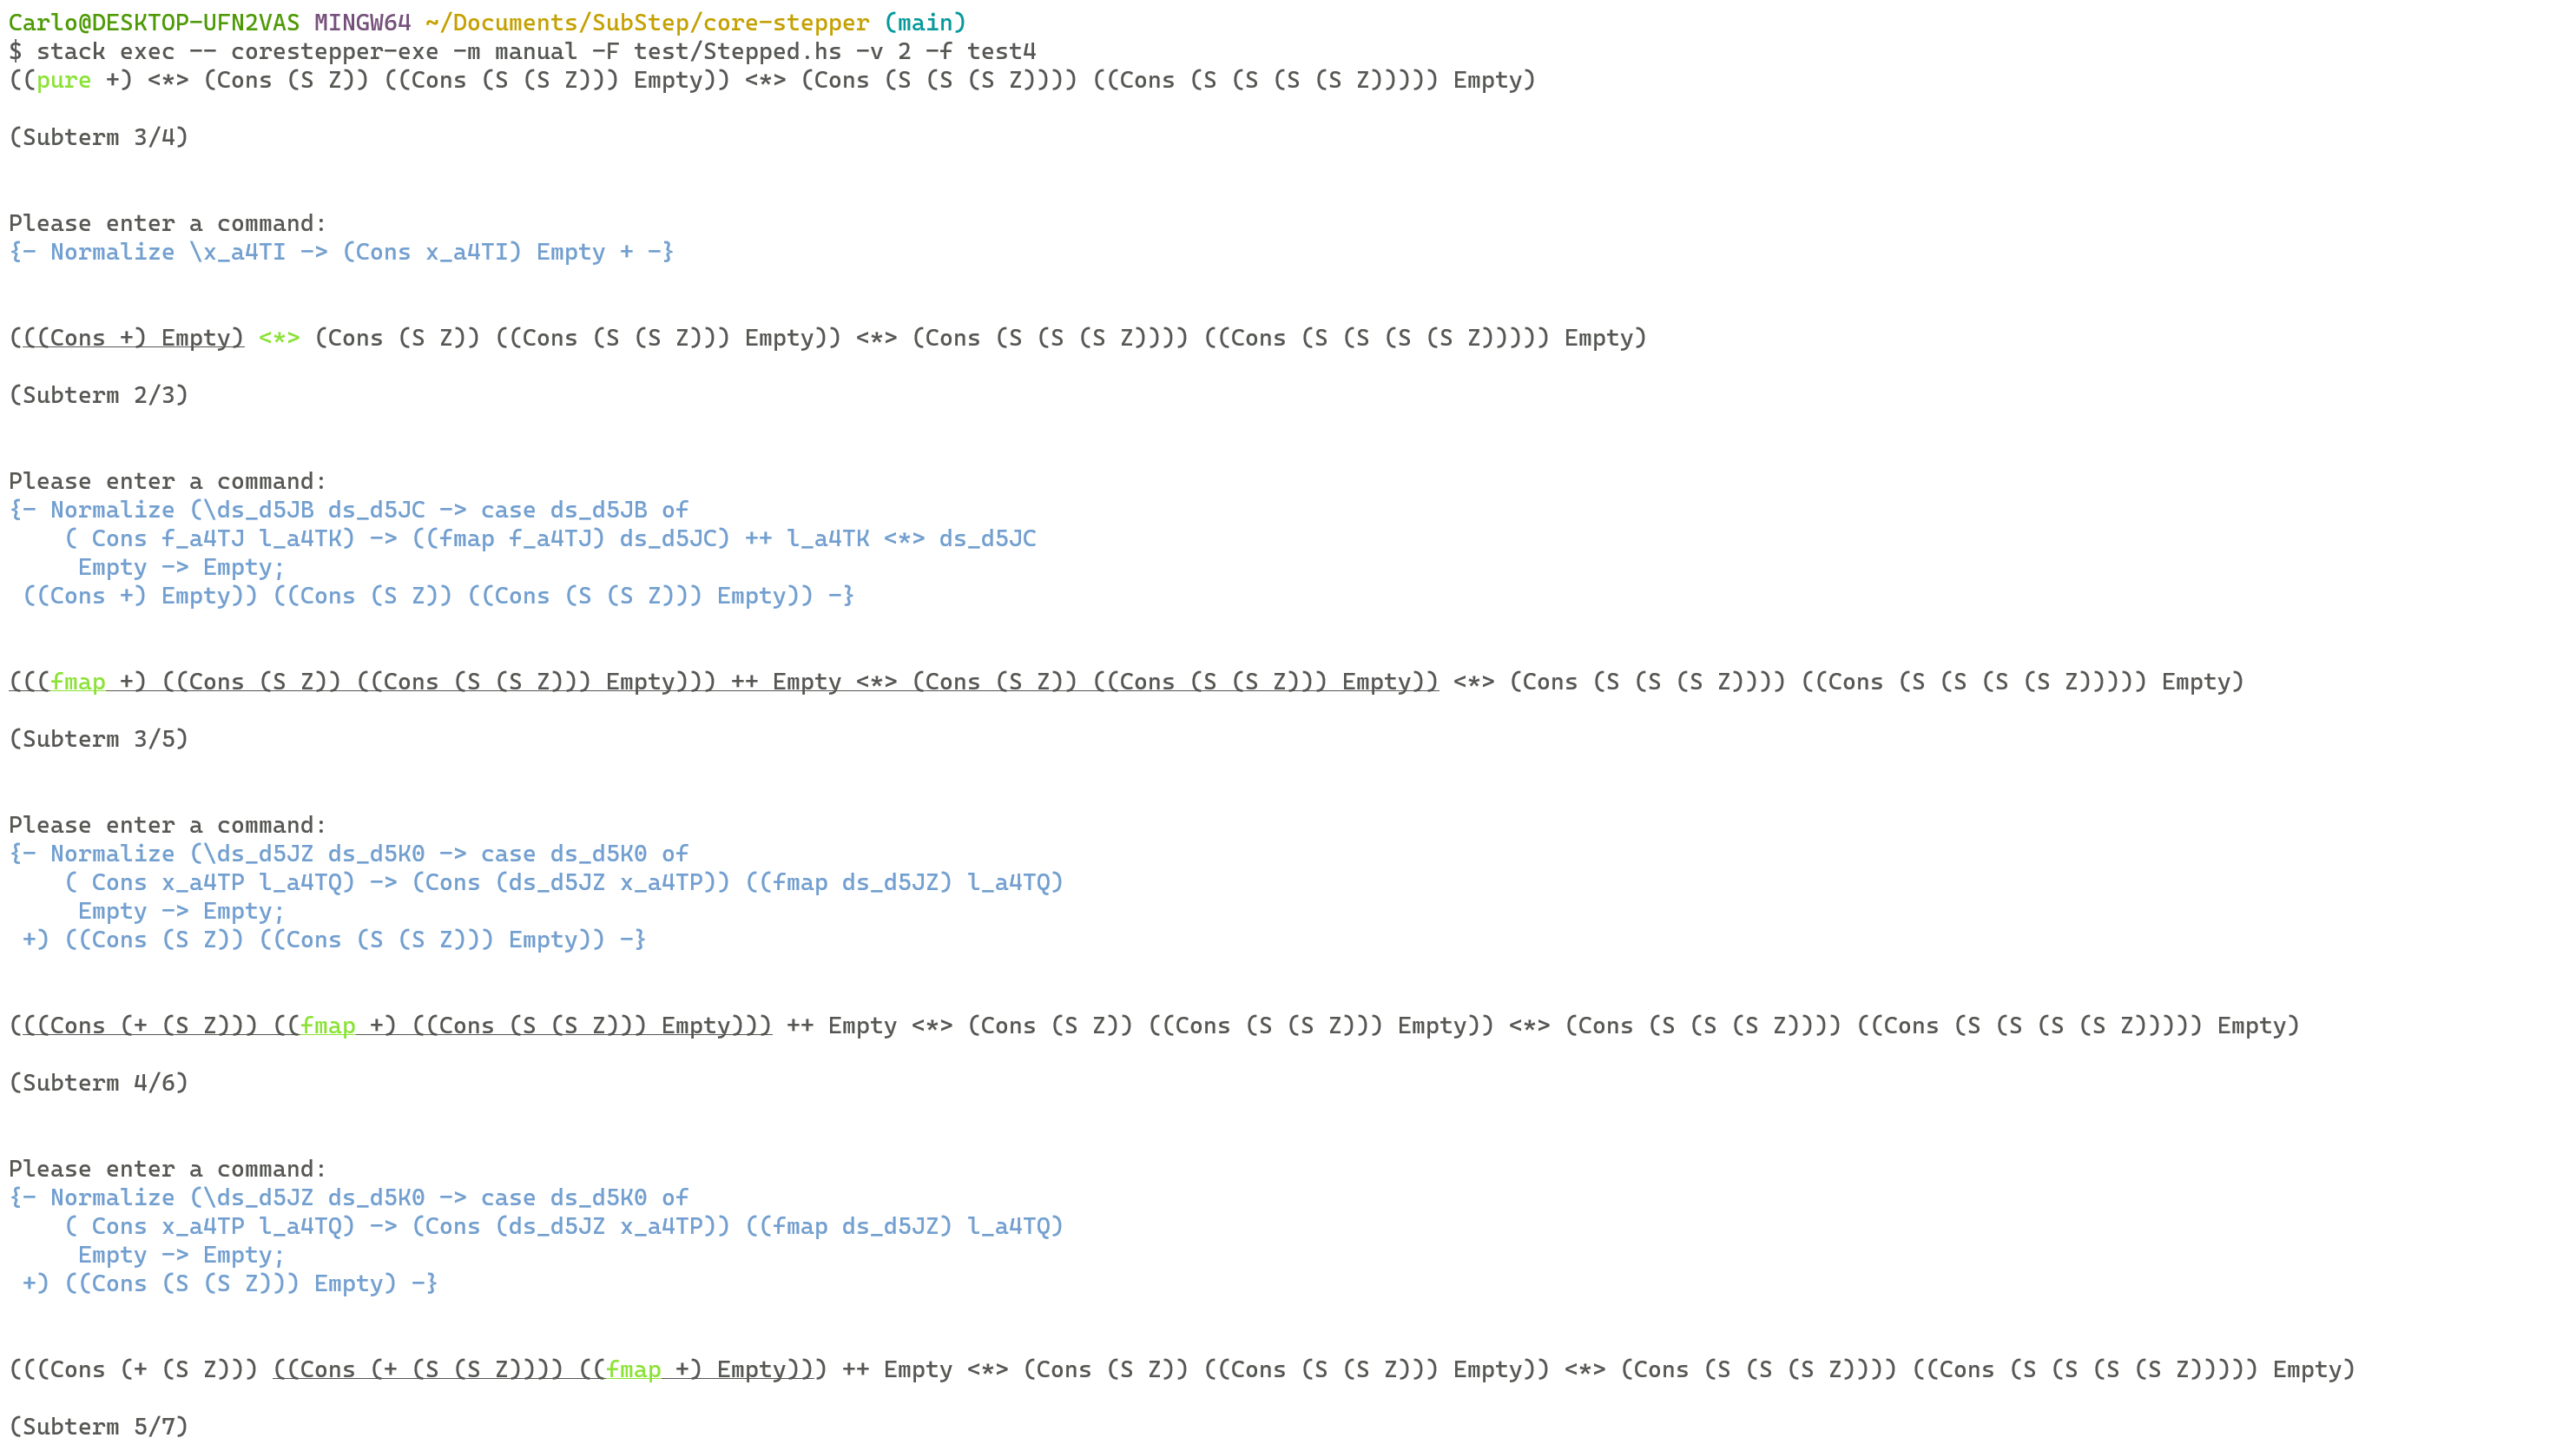
\includegraphics[width=1\textwidth]{resources/applicative_part_1.PNG}
\end{figure}
\begin{figure}
    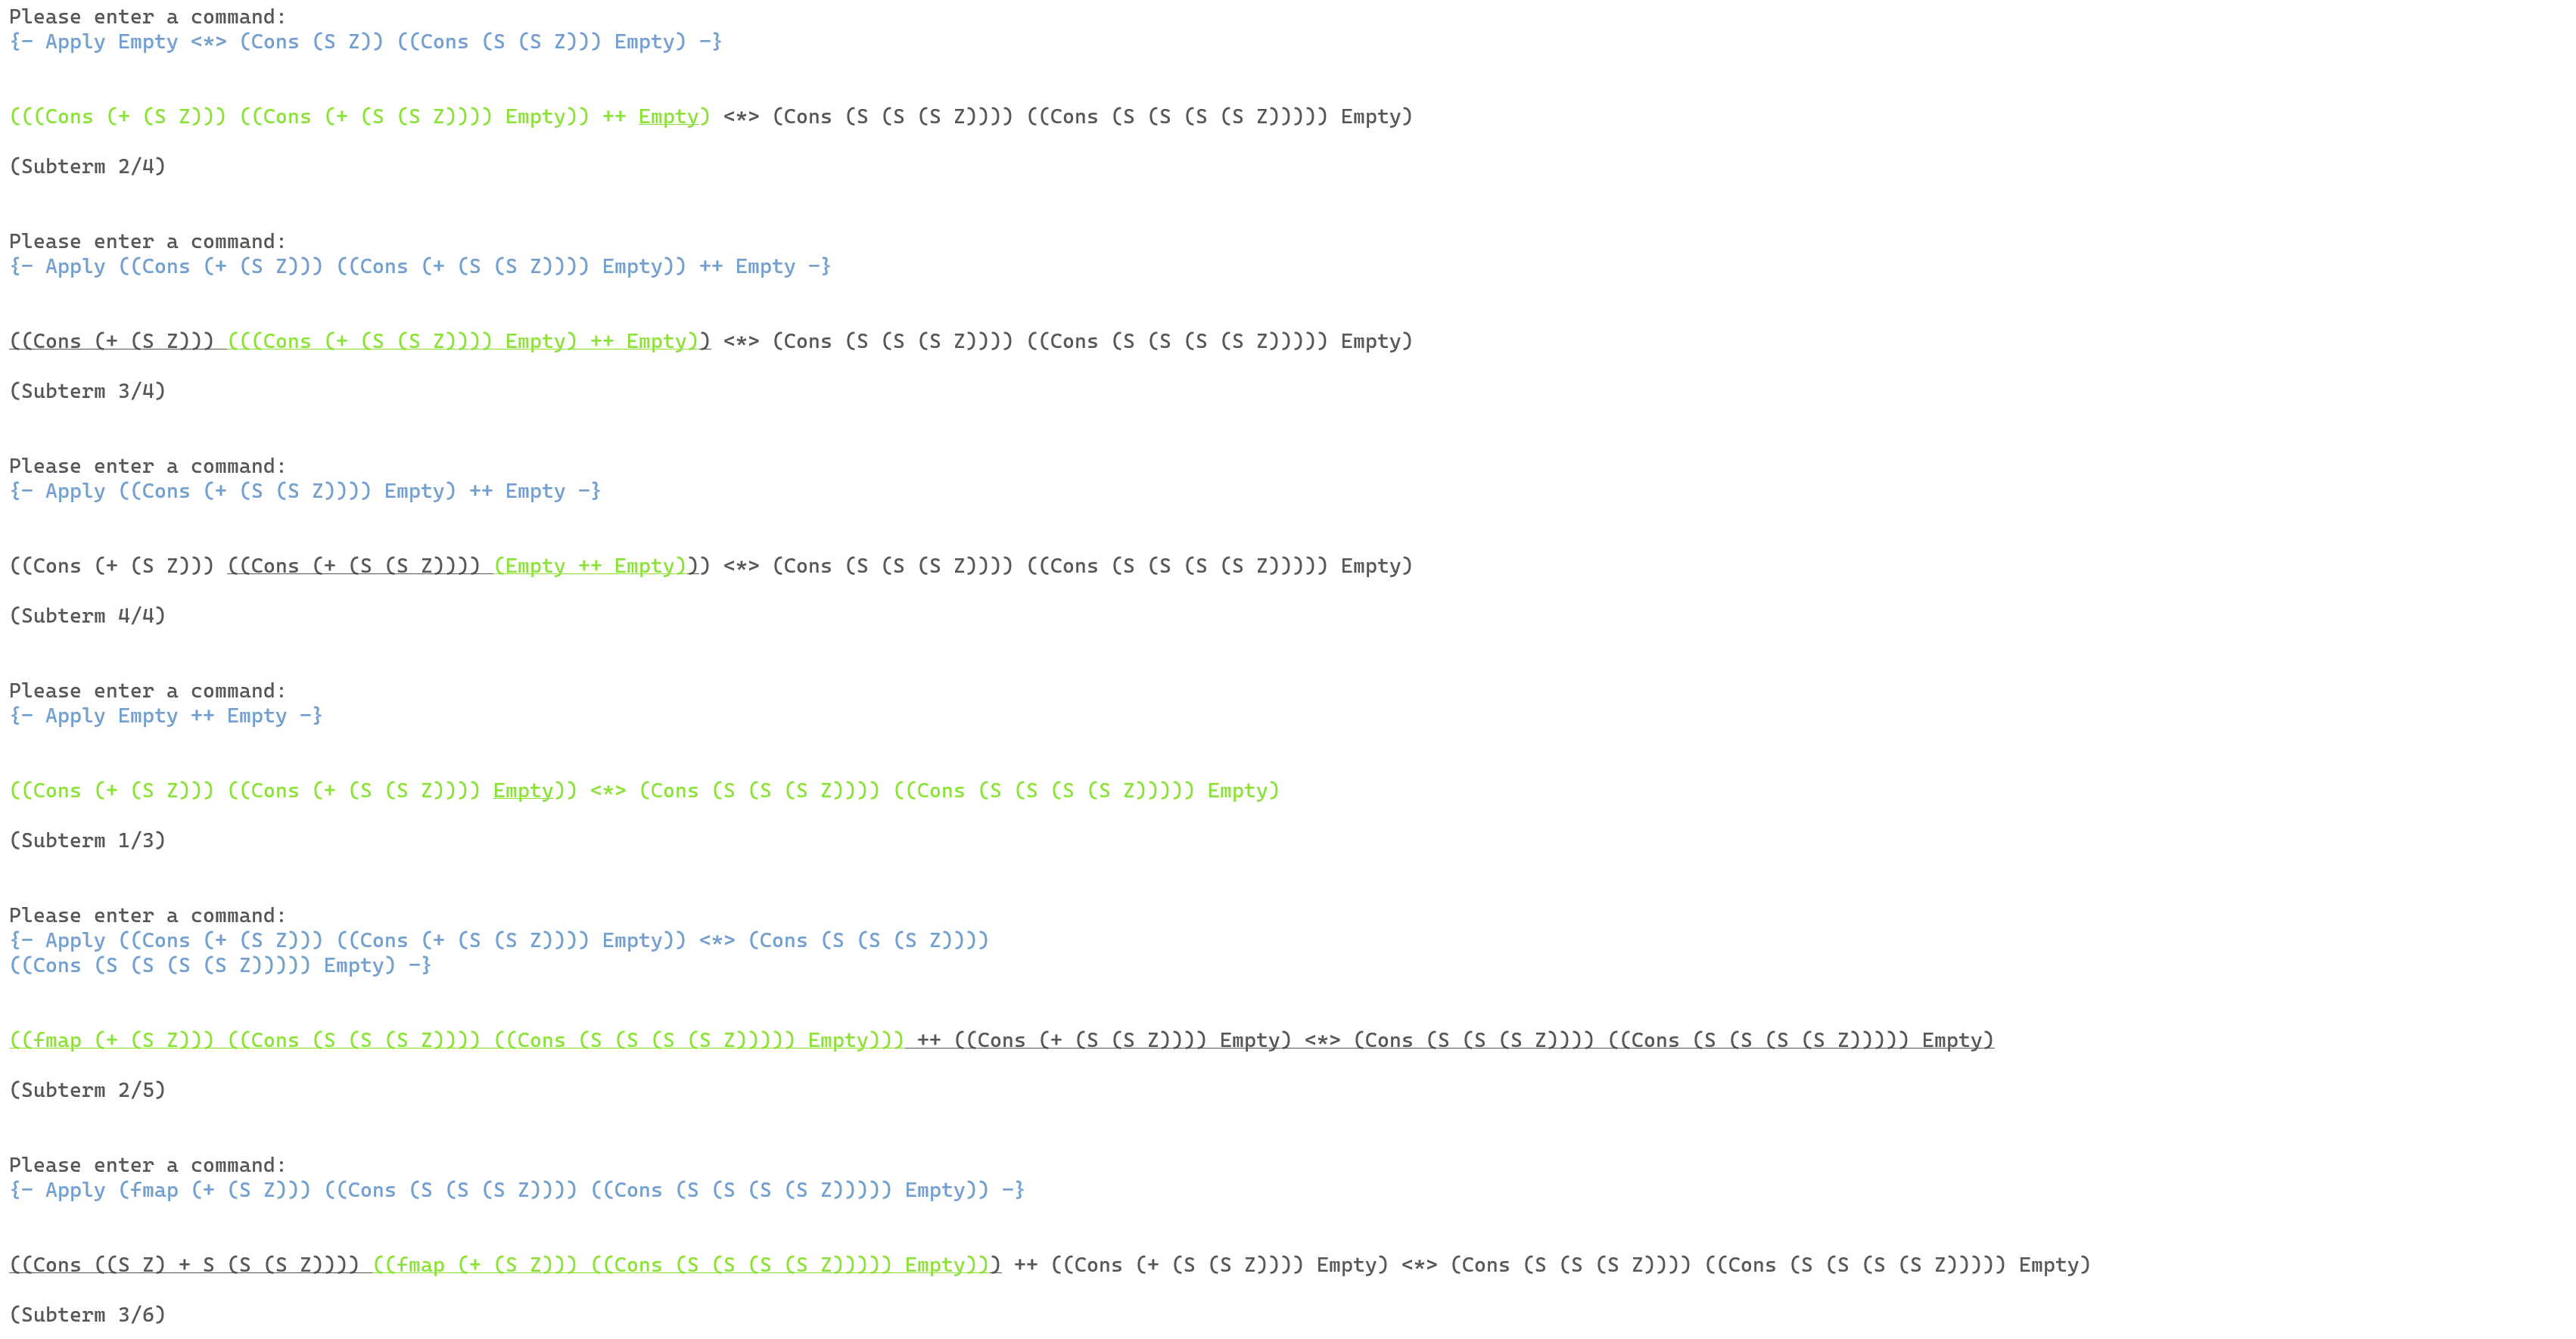
\includegraphics[width=1\textwidth]{resources/applicative_part_2.PNG}
\end{figure}
\begin{figure}
    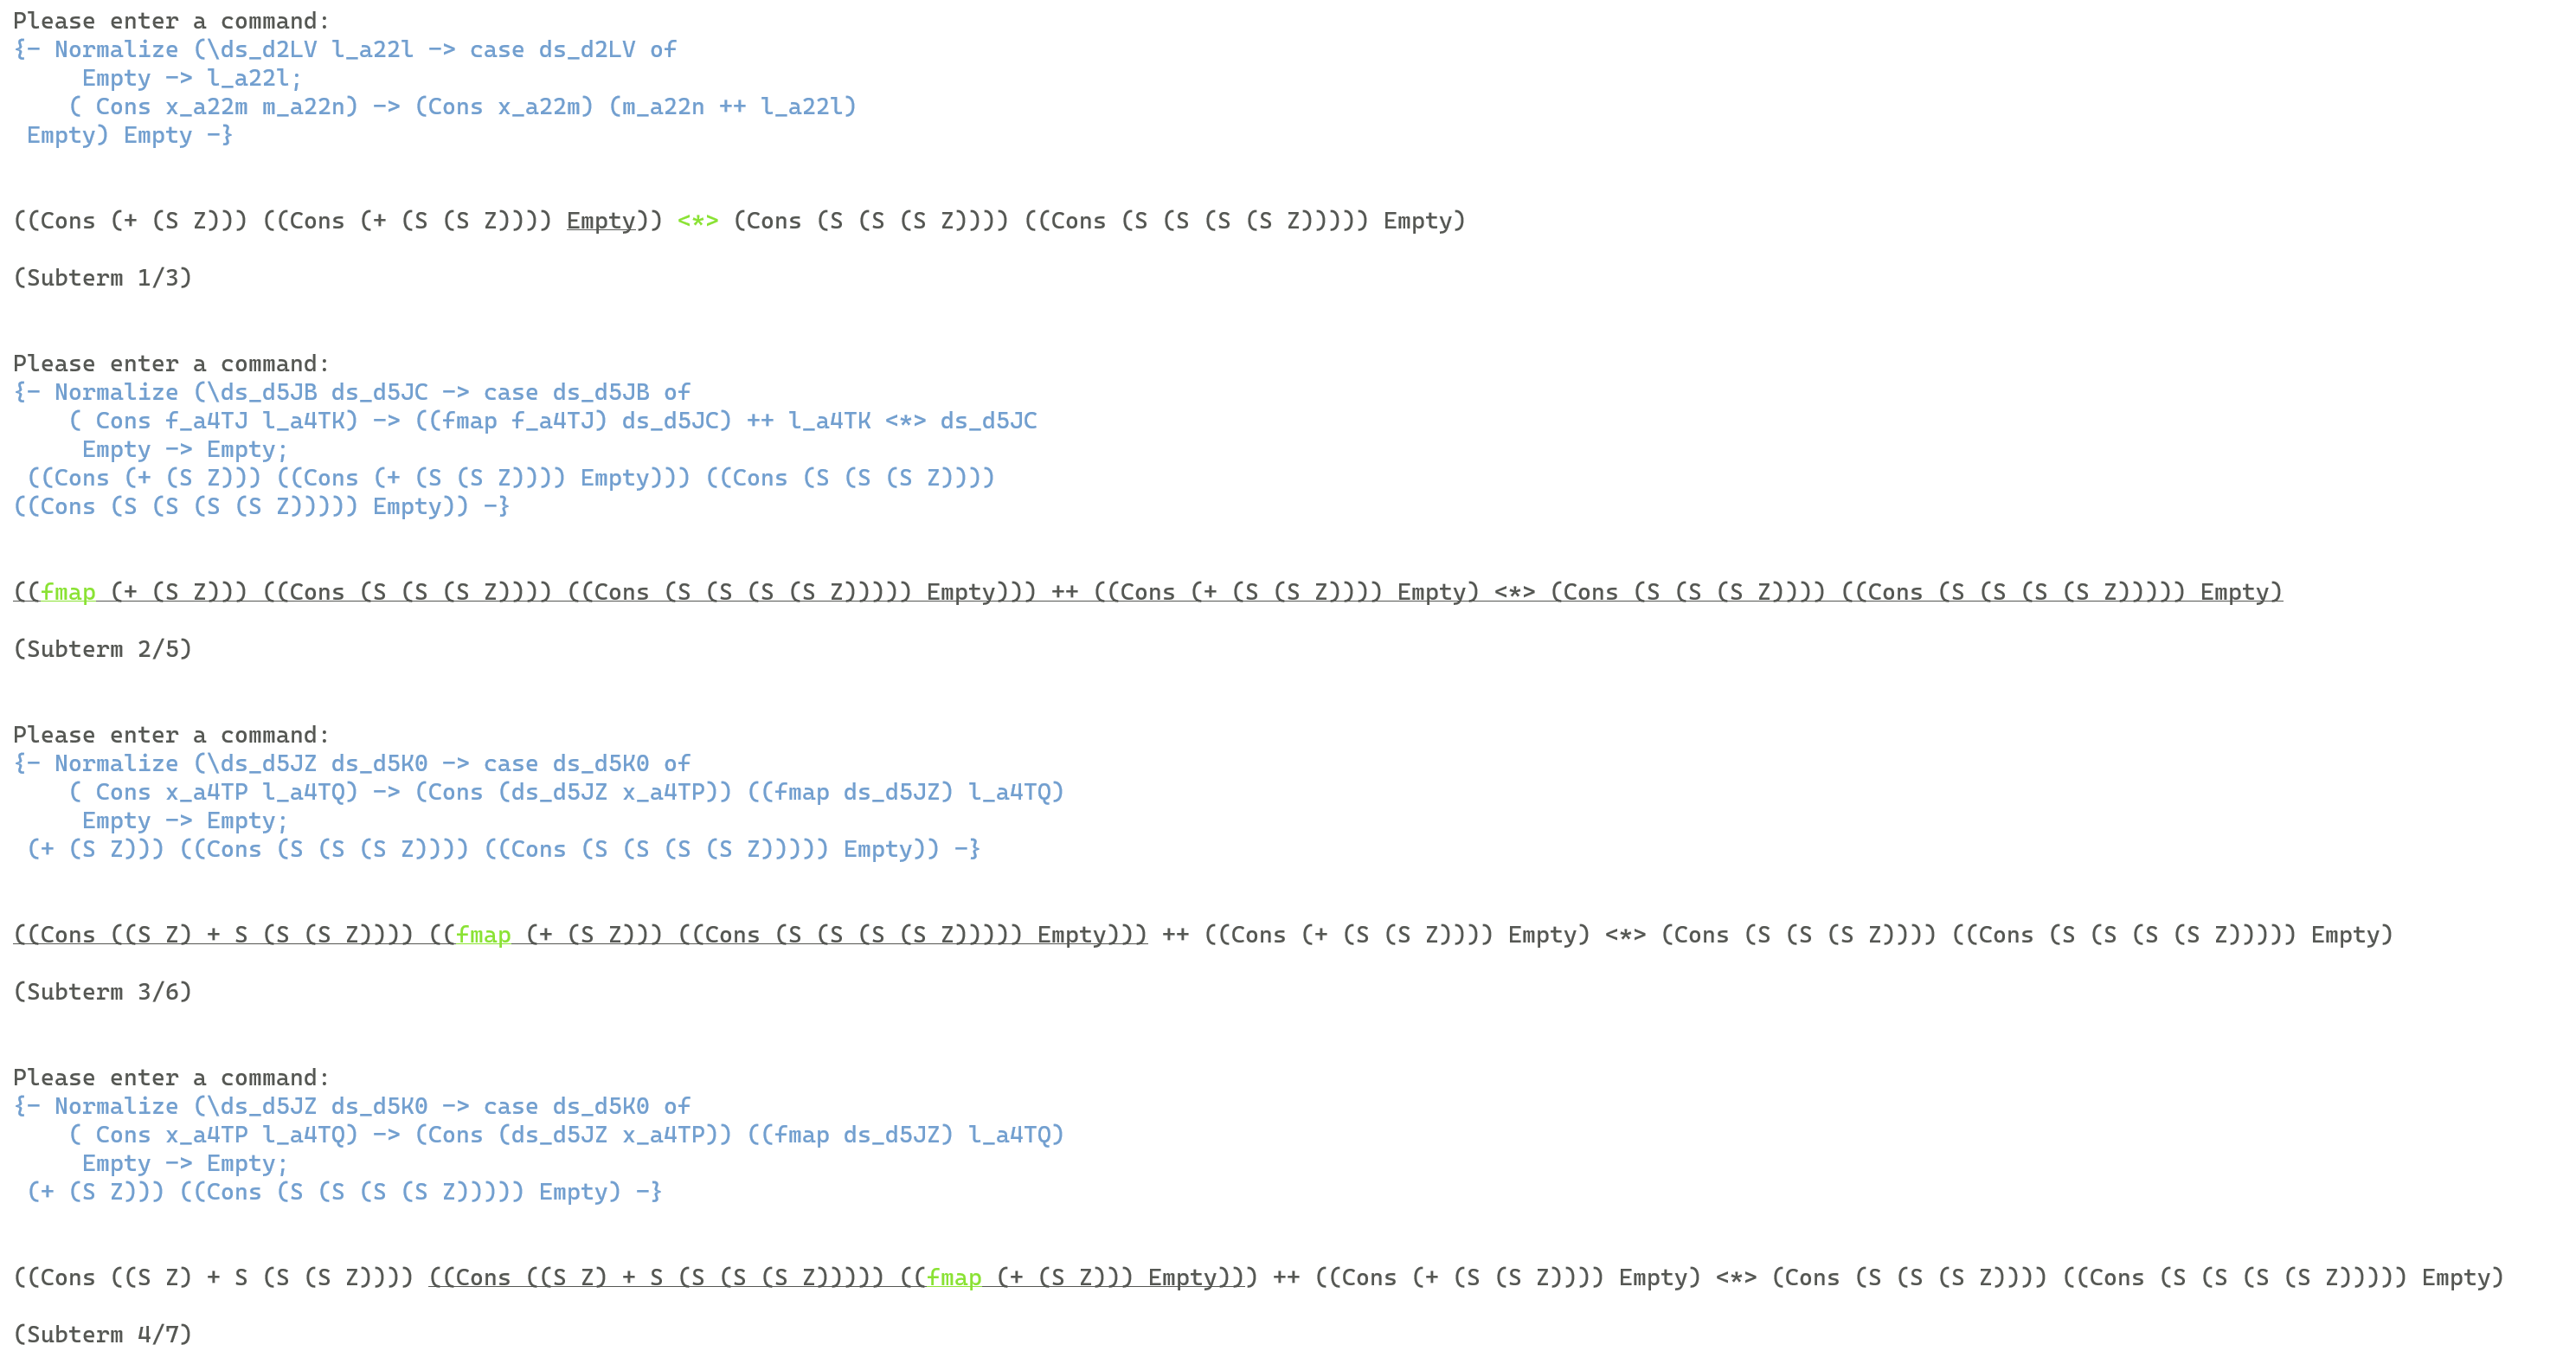
\includegraphics[width=1\textwidth]{resources/applicative_part_3.PNG}
\end{figure}
\begin{figure}
    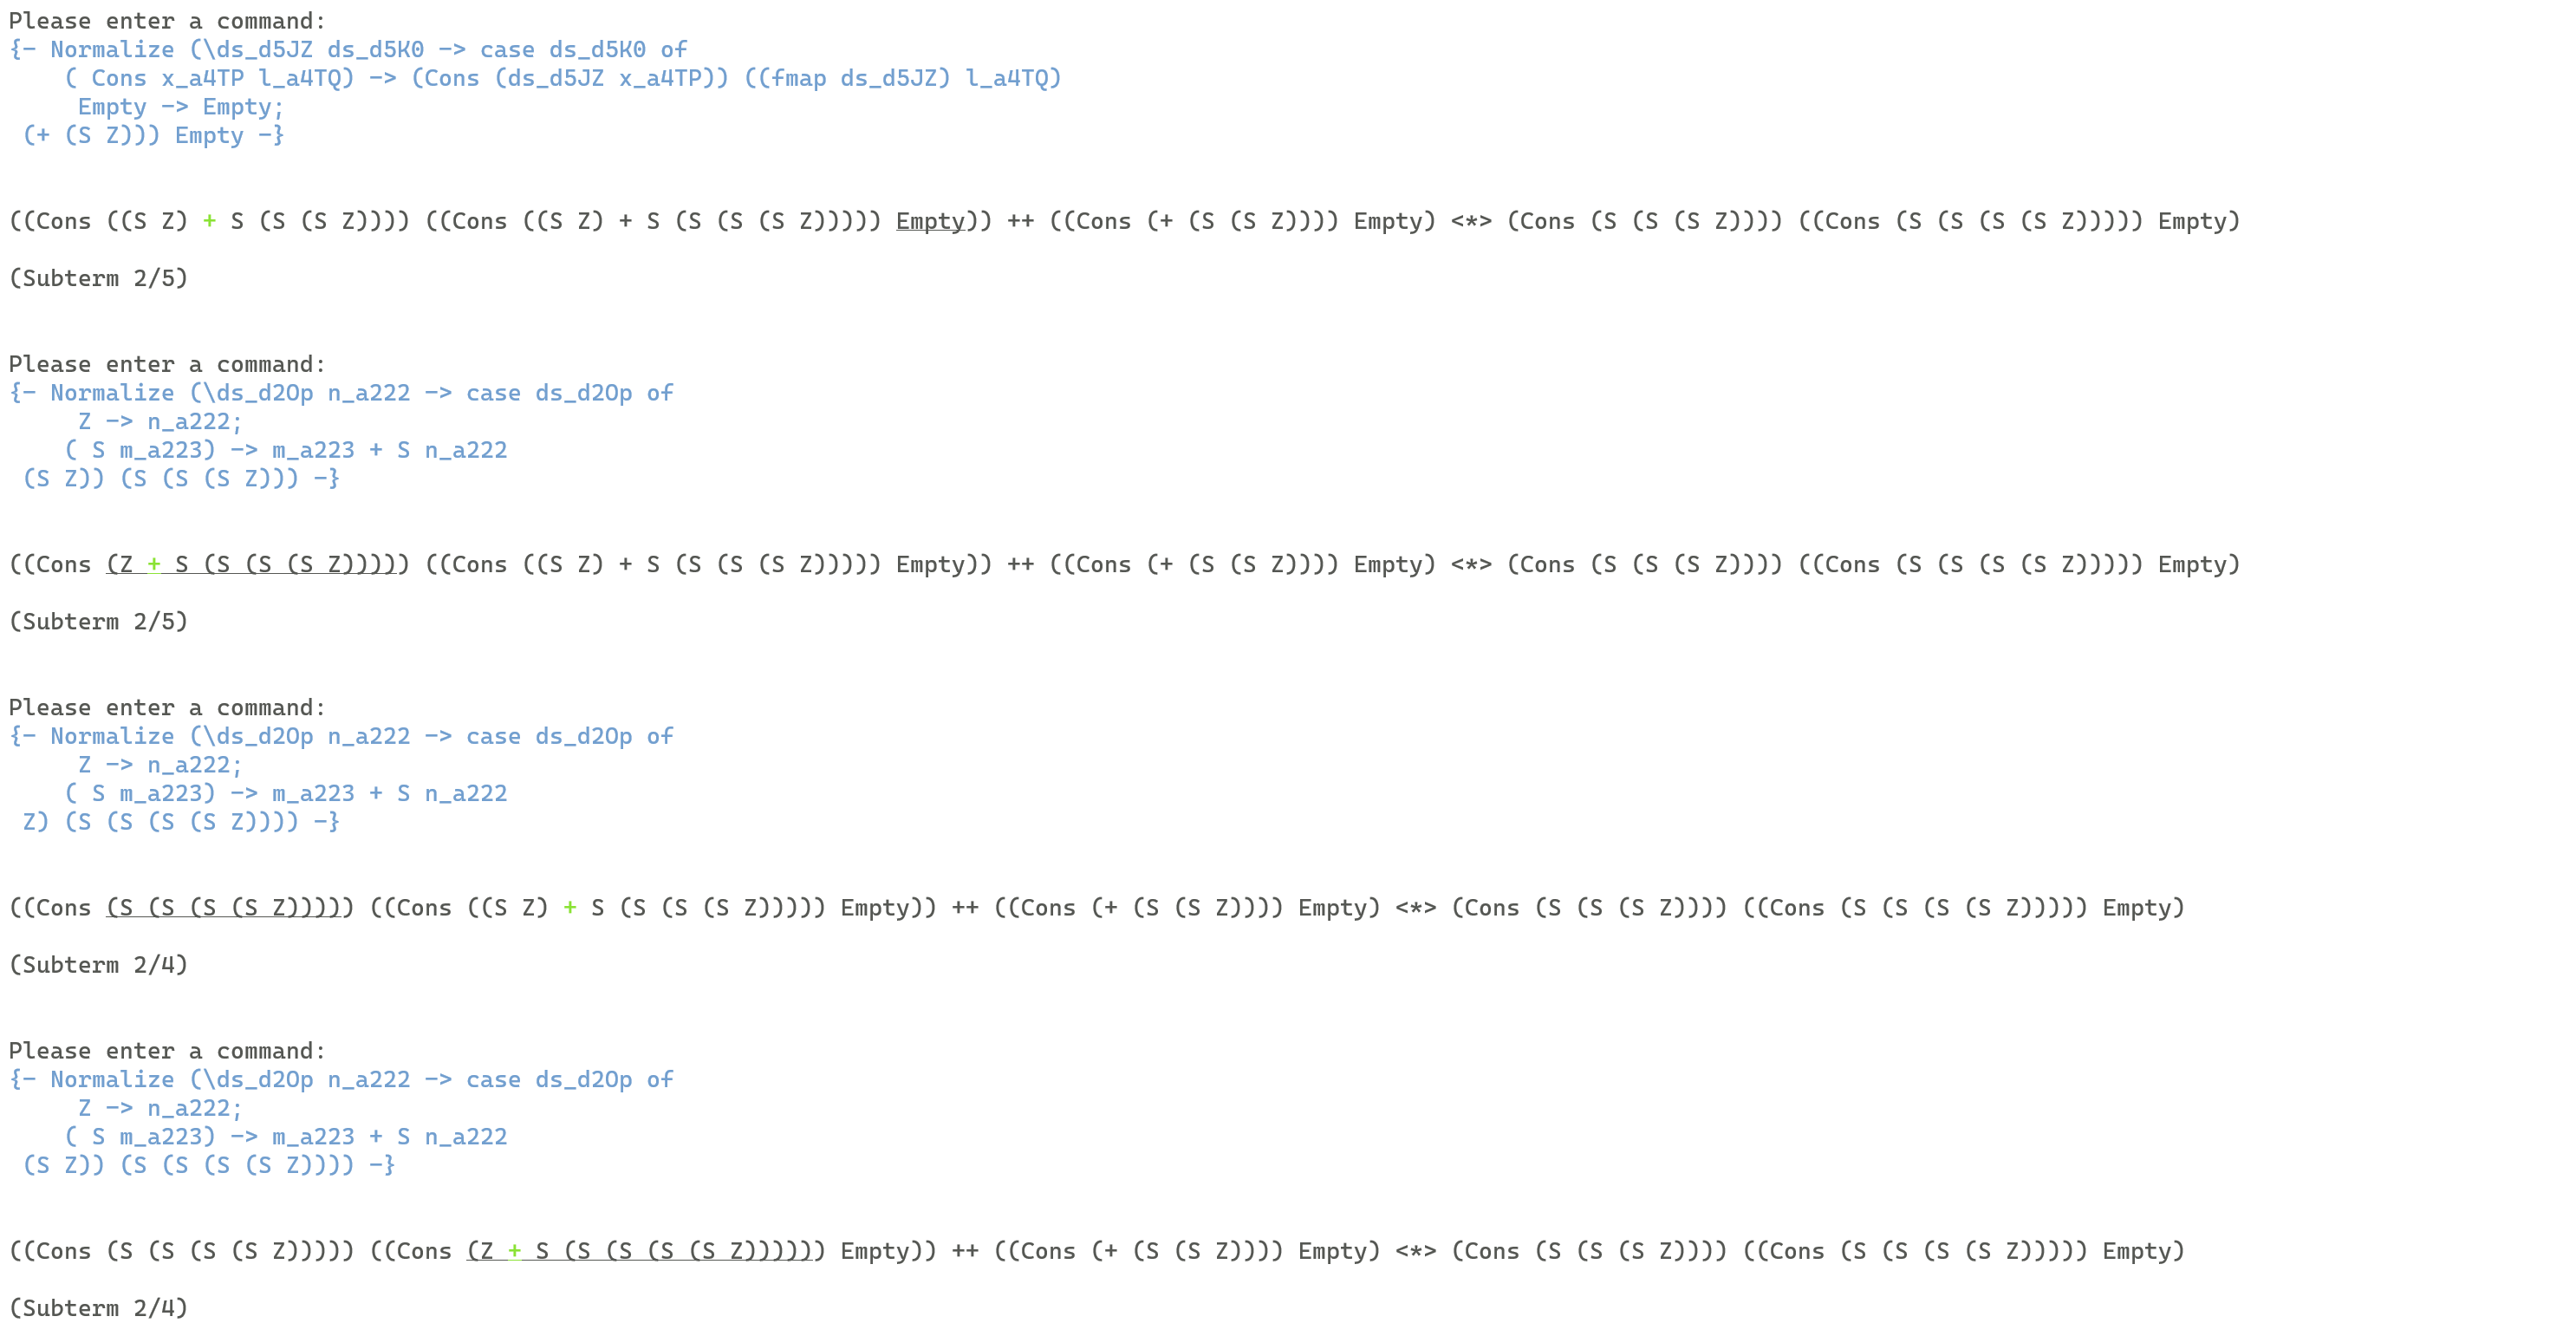
\includegraphics[width=1\textwidth]{resources/applicative_part_4.PNG}
\end{figure}
\begin{figure}
    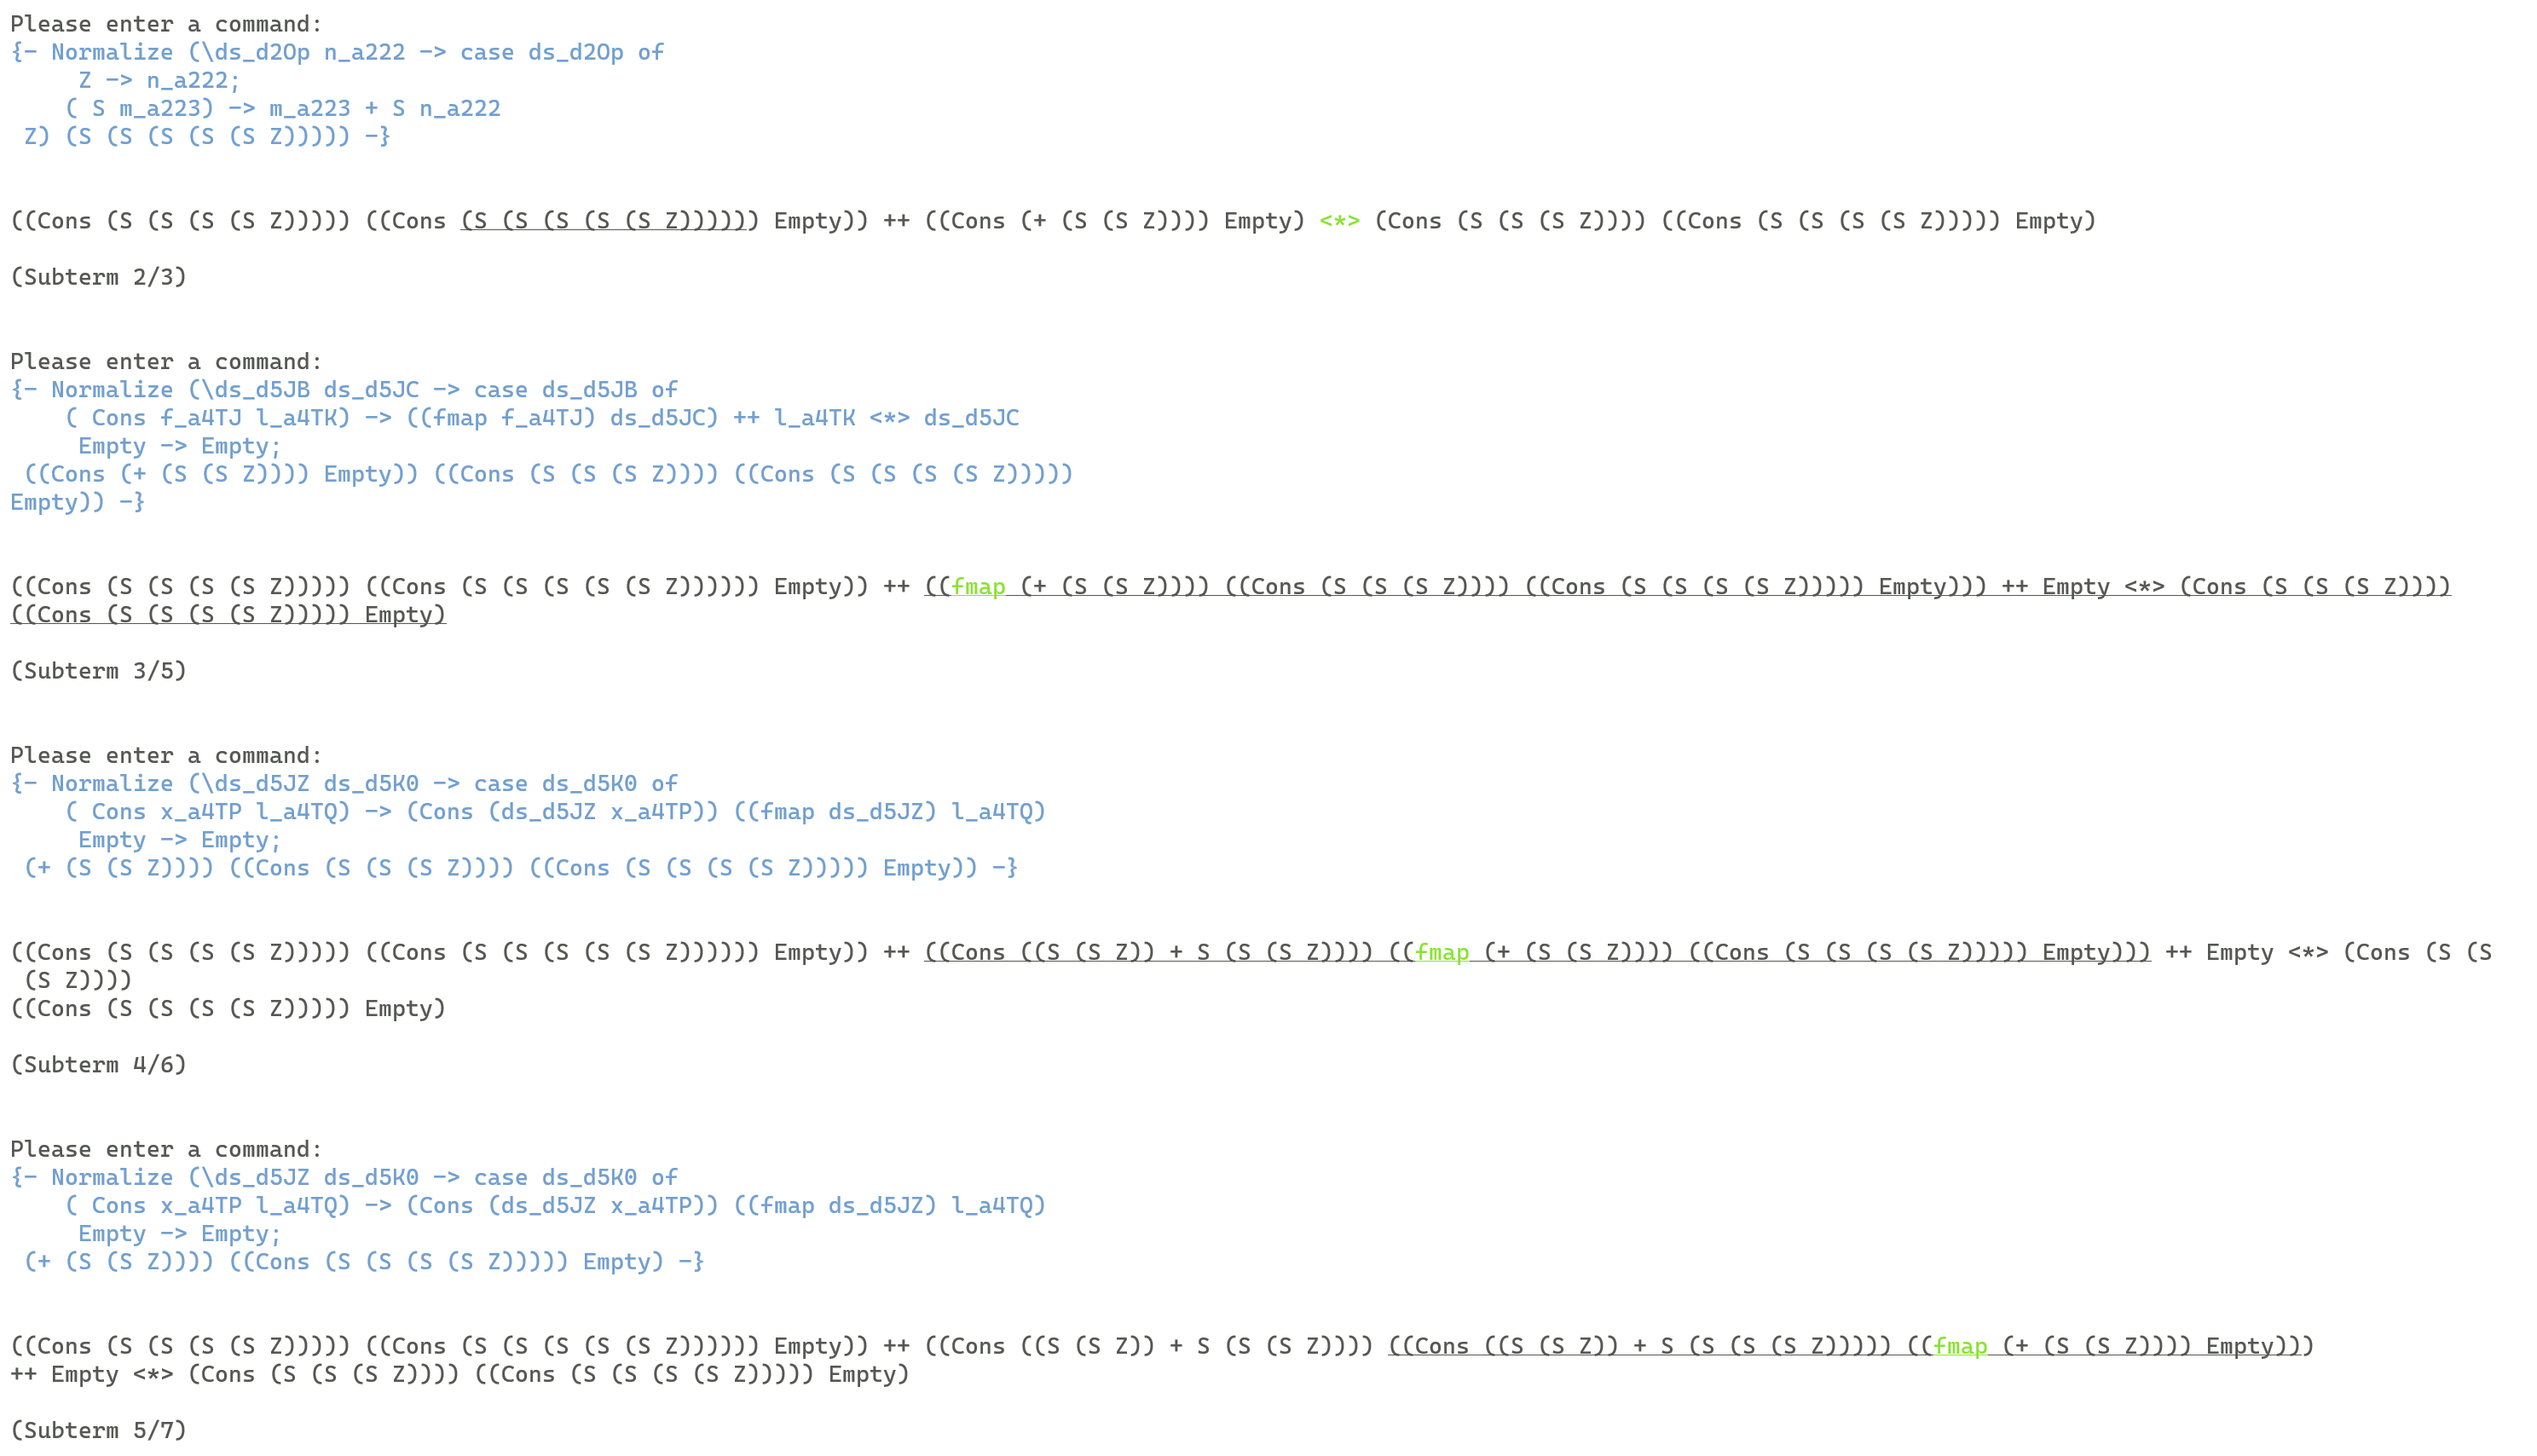
\includegraphics[width=1\textwidth]{resources/applicative_part_5.PNG}
\end{figure}
\begin{figure}
    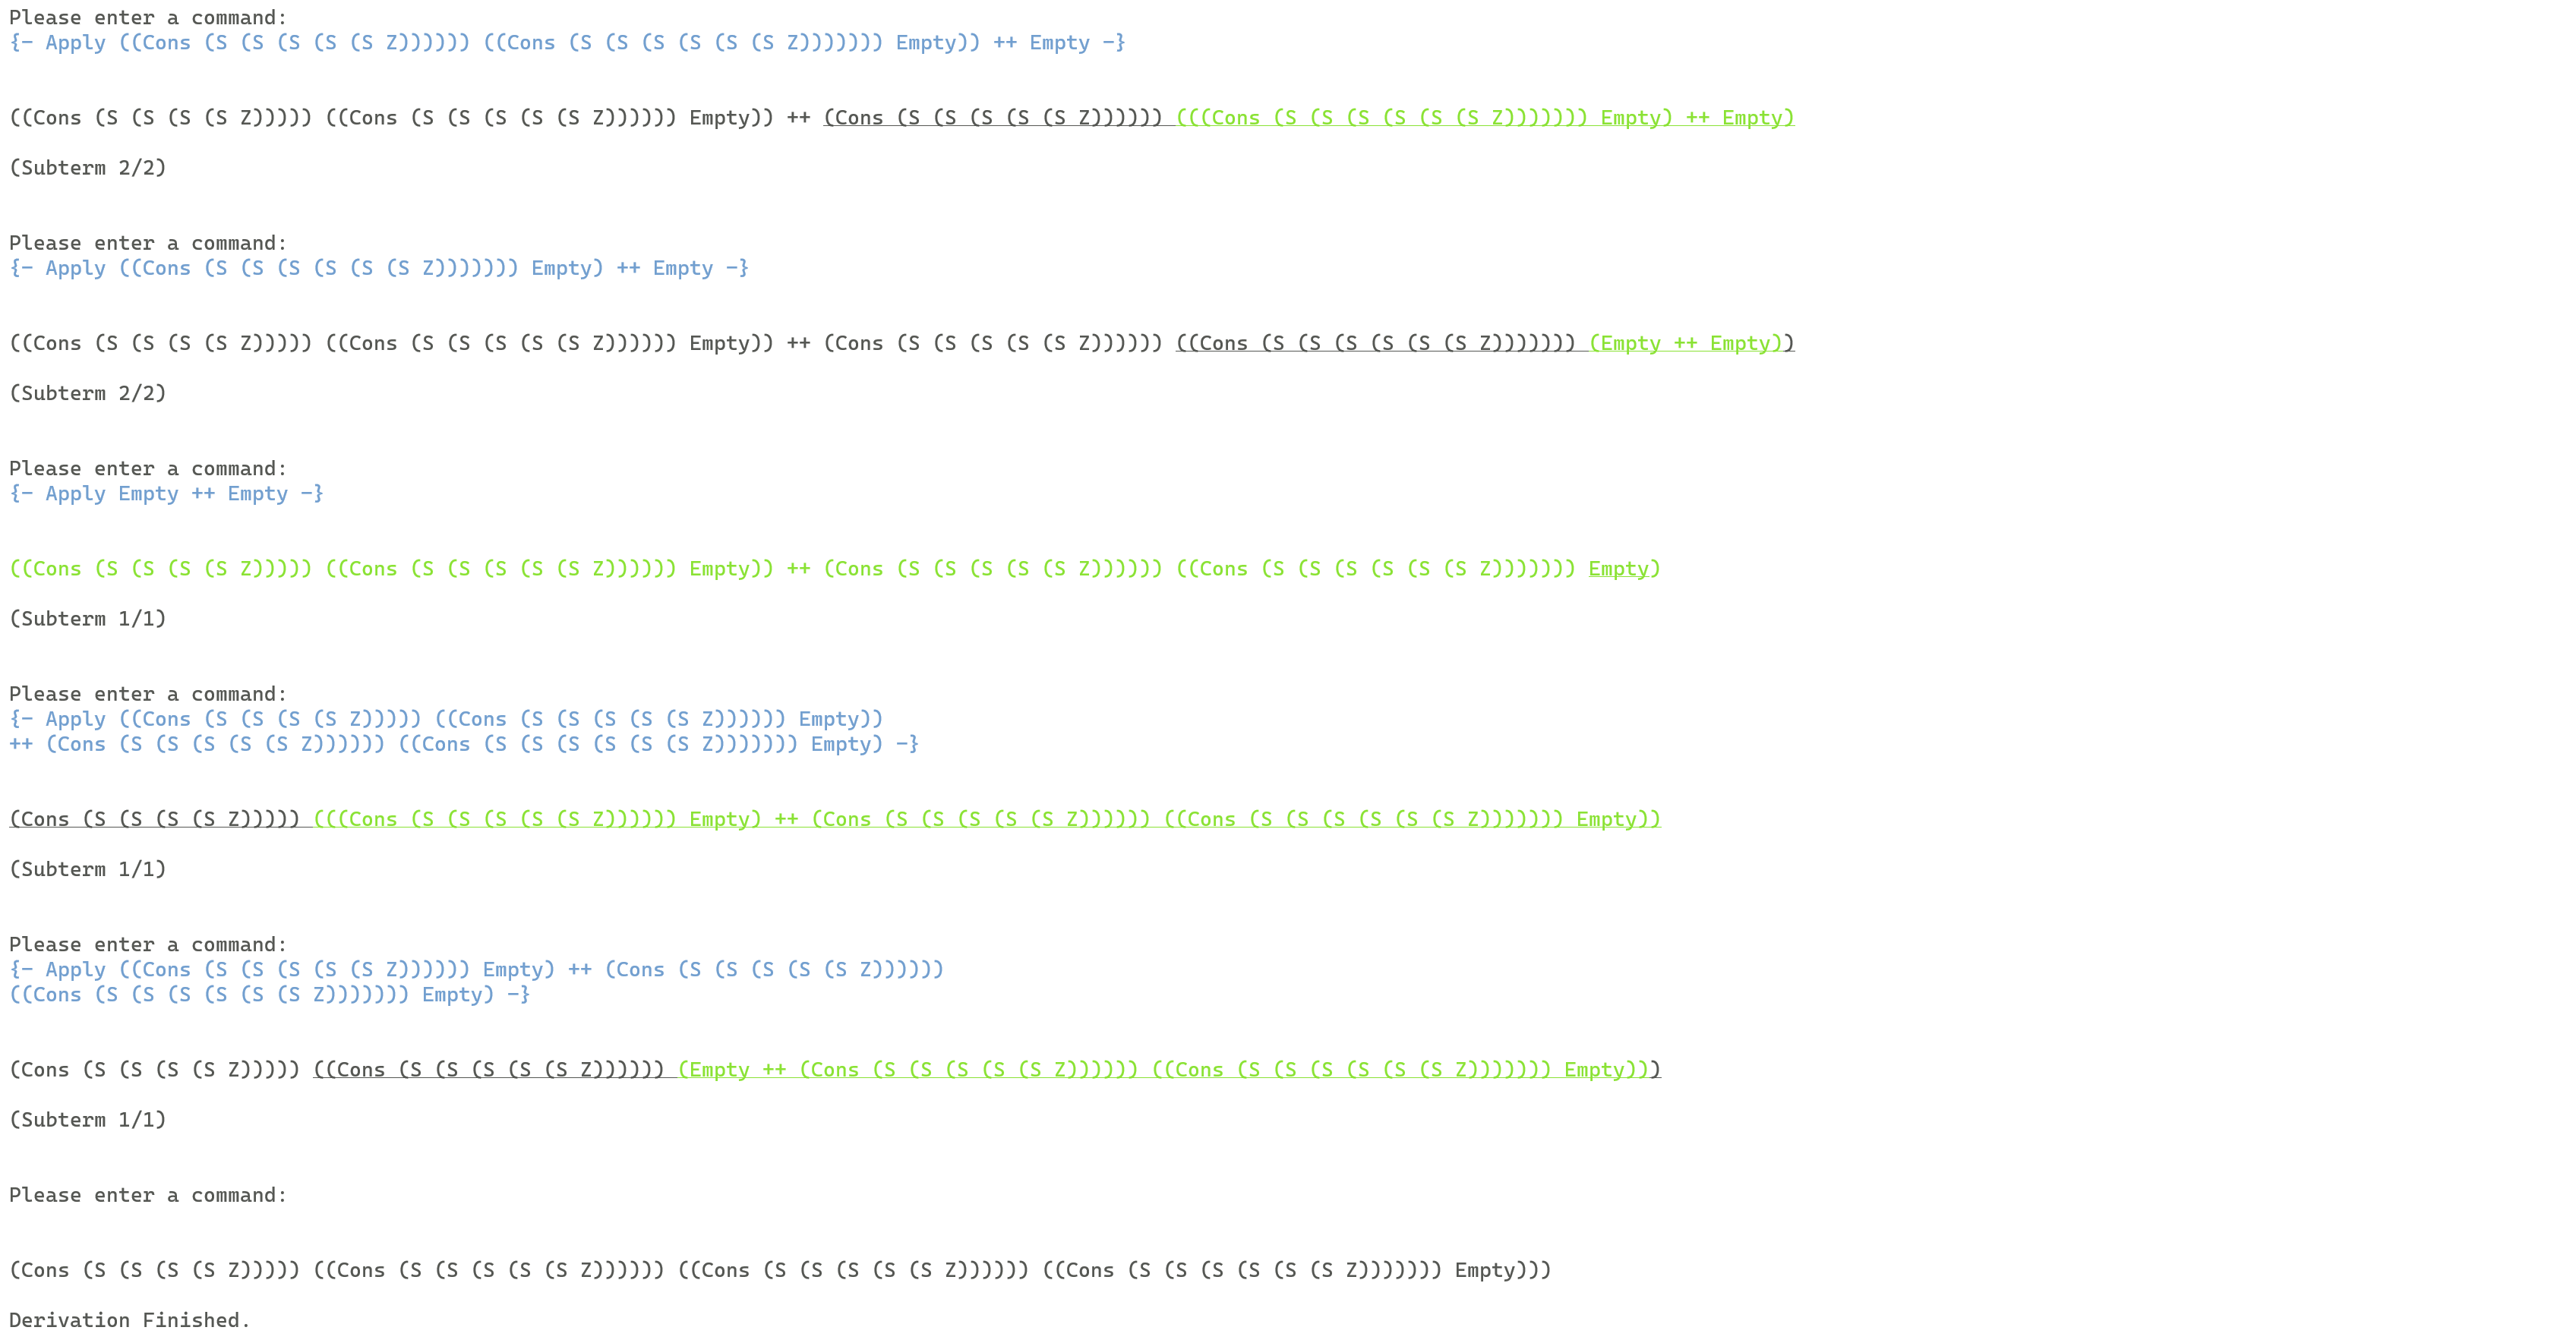
\includegraphics[width=1\textwidth]{resources/applicative_part_6.PNG}
    \caption{The third example, equivalent to \texttt{pure (+) <*> [1,2] <*> [3,4]}}
\end{figure}


\clearpage
\section{Example 4}
The fourth example needed to make a slightly bigger change again,
since it is using the Nat datatype as well.
Since division is harder to implement on the Nat datatype,
I have chosen to perform a subtraction instead.
Similar to the division for the Int datatype,
the subtraction for the Nat datatype can cause an error as well,
if a bigger number is subtracted from a smaller number (negative number error).

Because of this,
the fourth example here is pretty much equivalent to the example in the task description,
even though different operations and datatypes are used.

\begin{figure}
    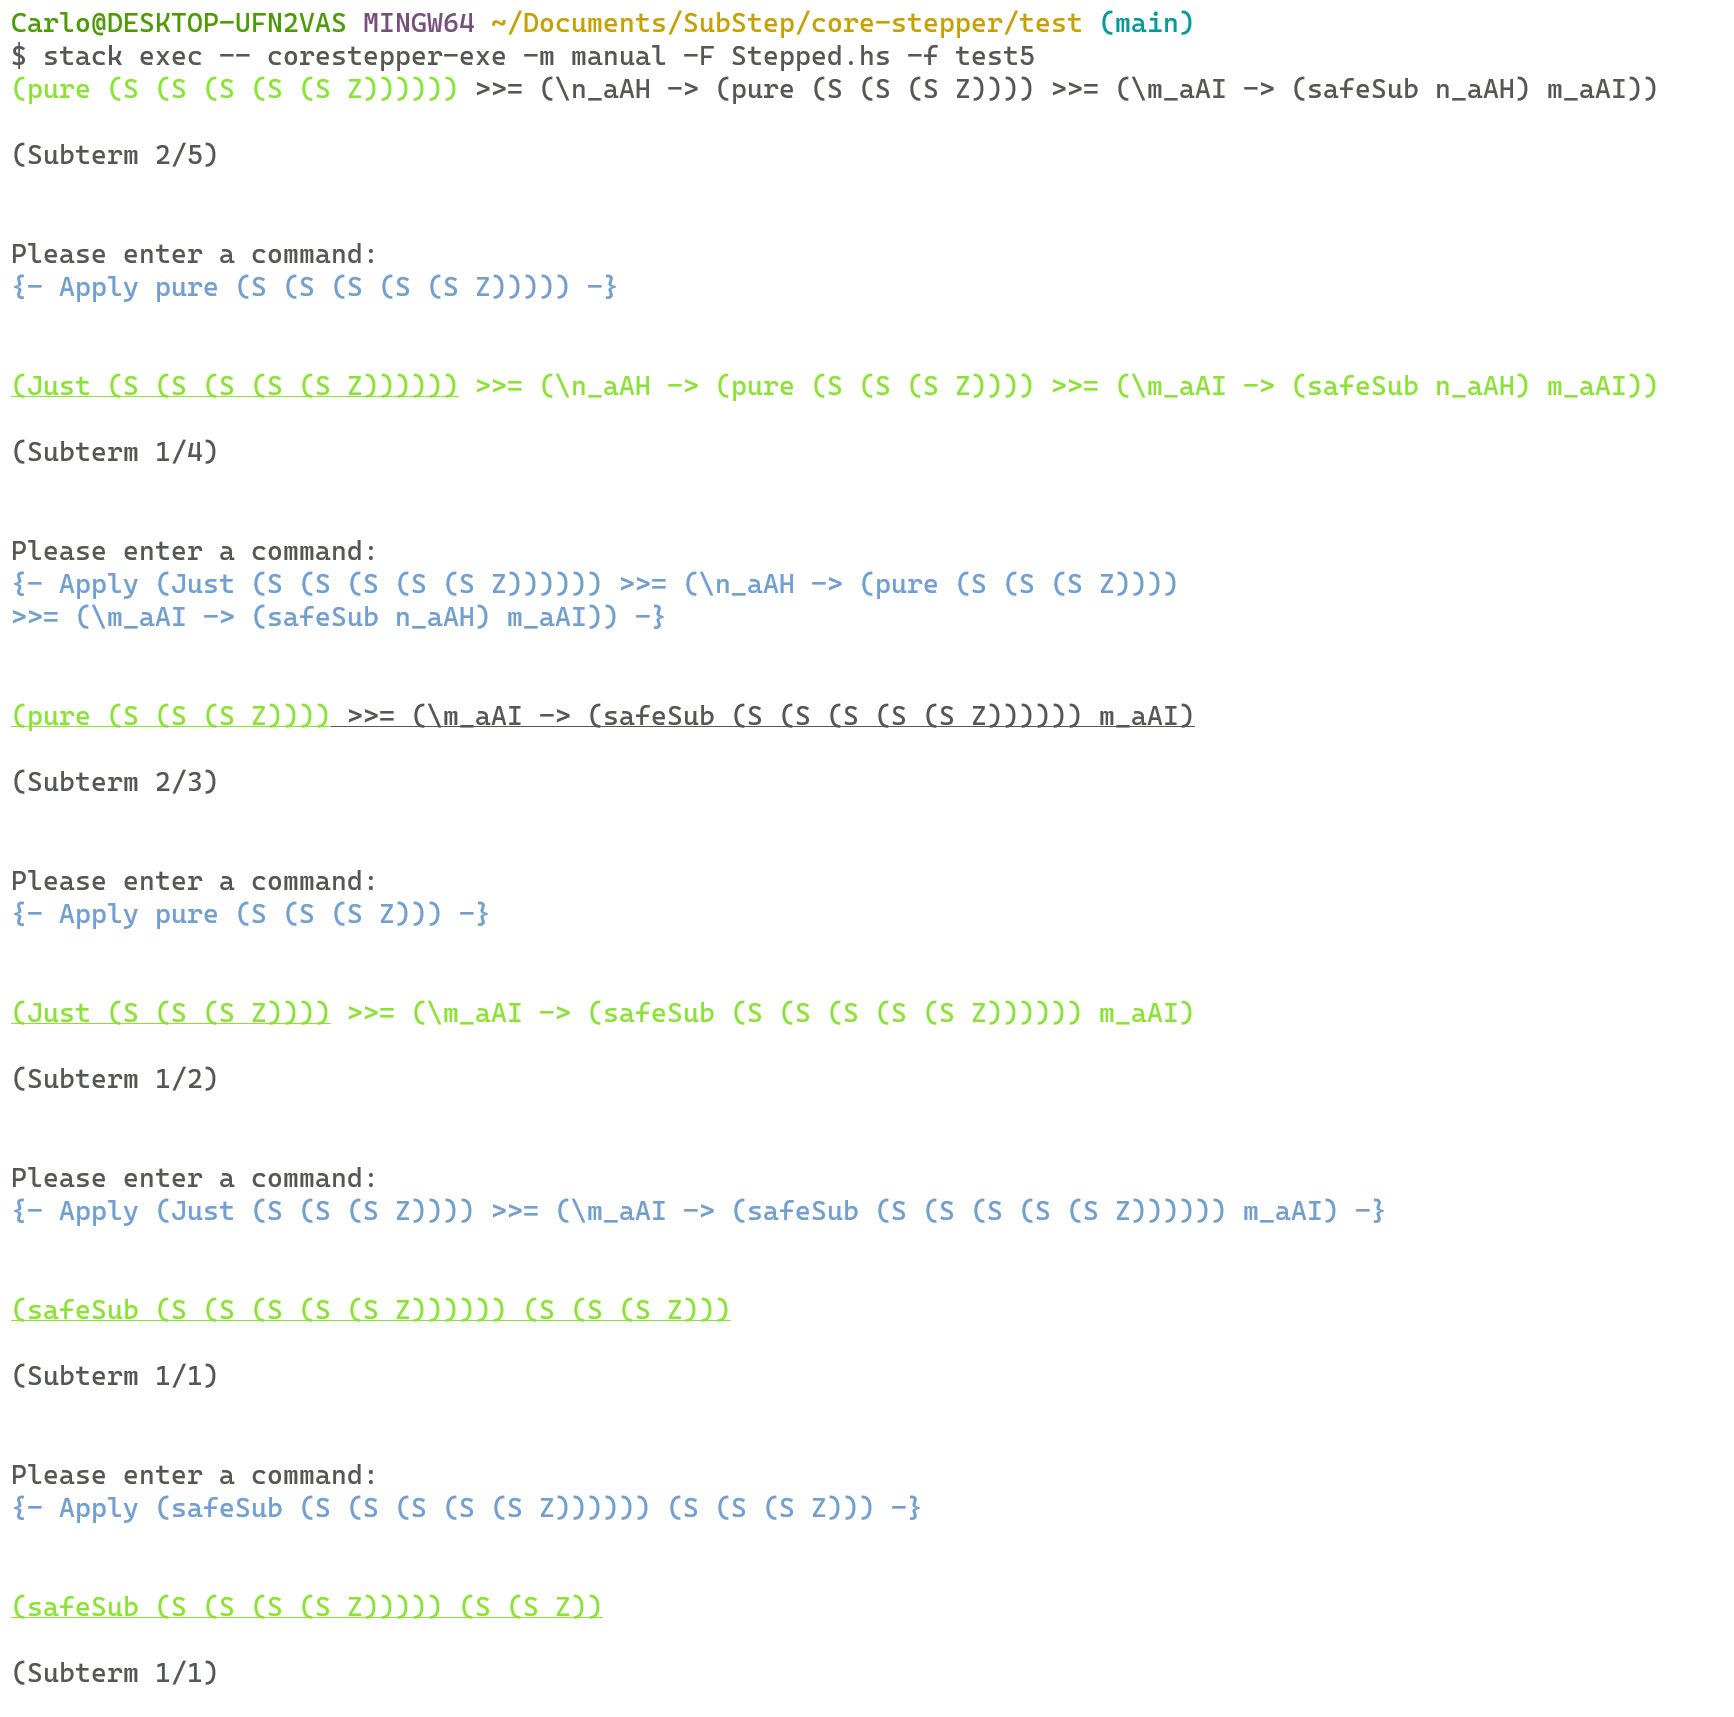
\includegraphics[width=1\textwidth]{resources/bind_part_1.PNG}
\end{figure}
\begin{figure}
    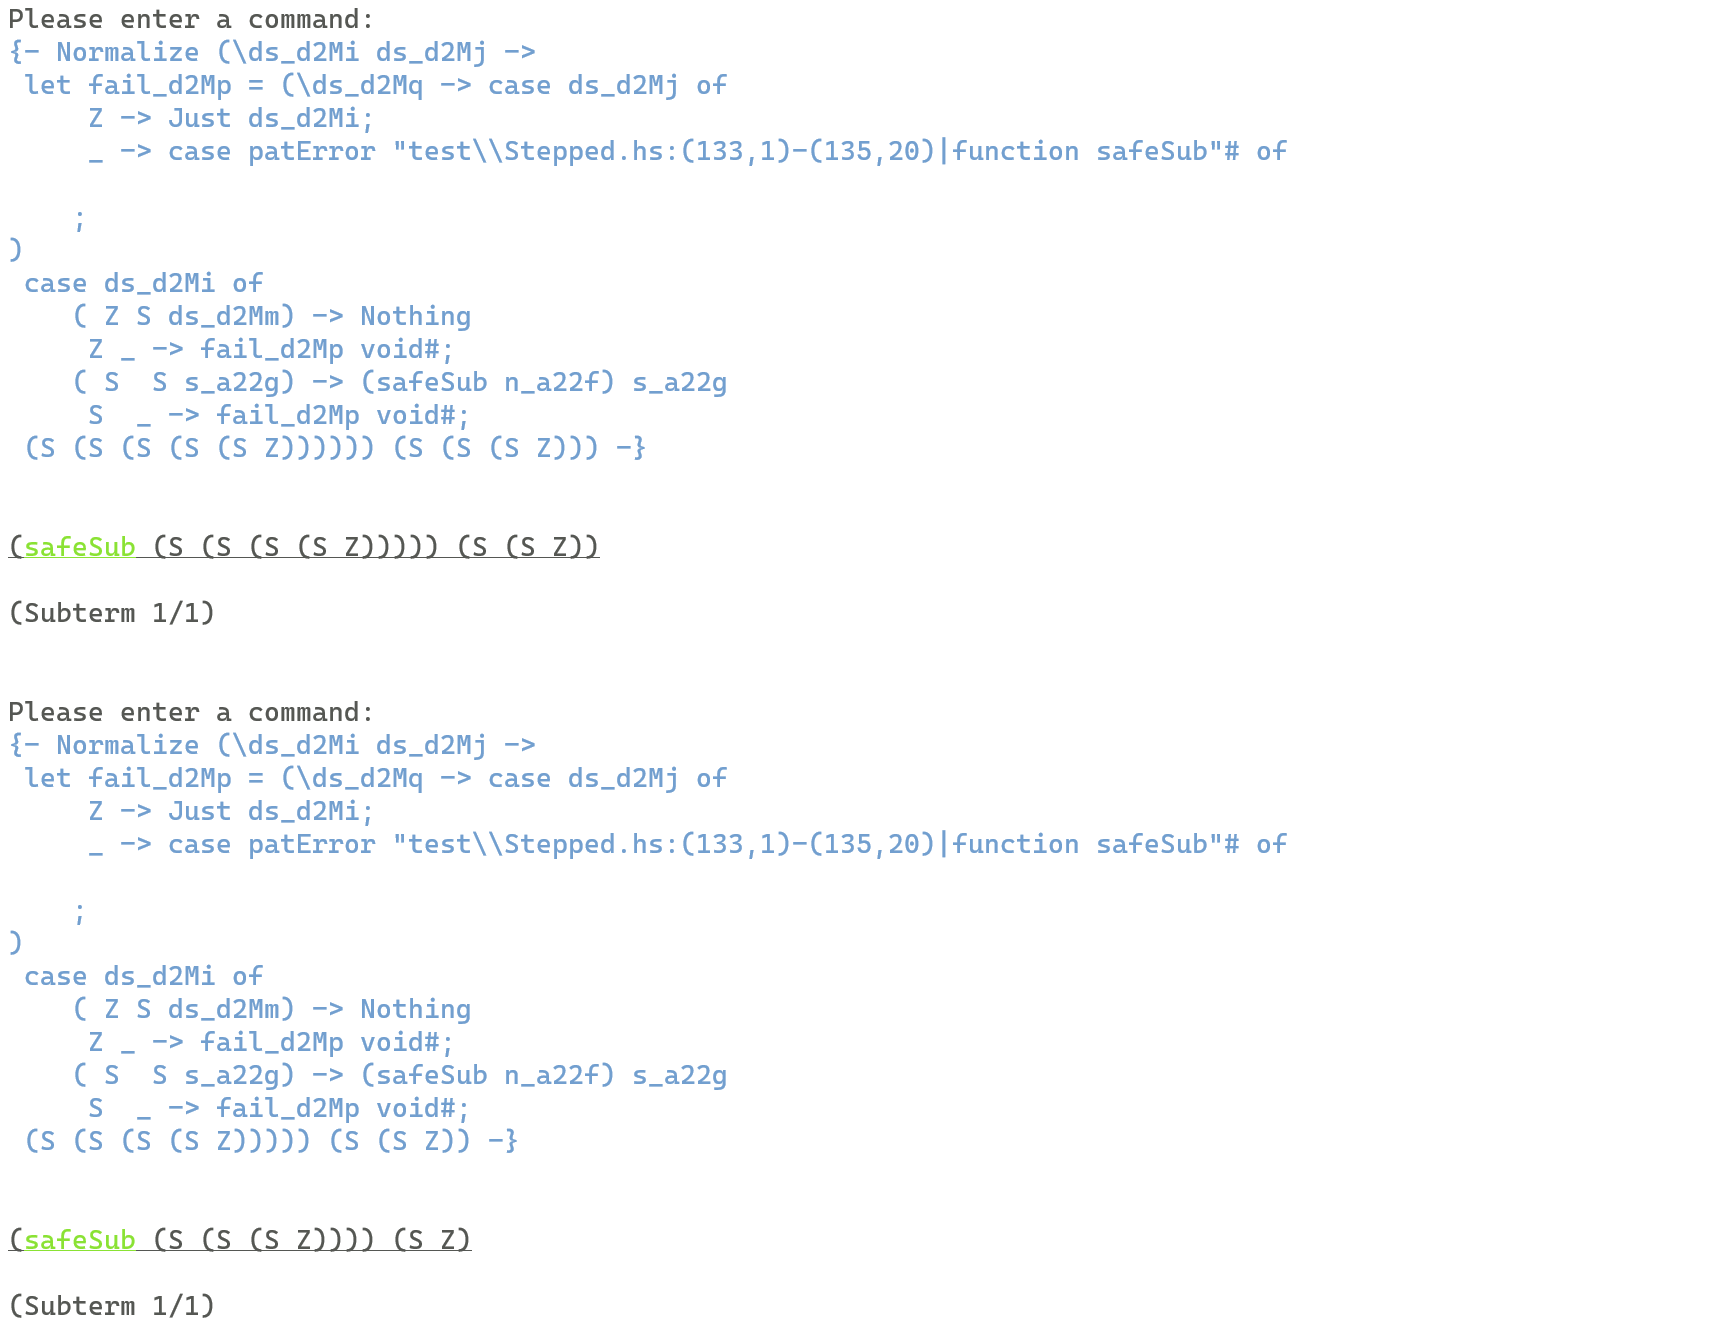
\includegraphics[width=1\textwidth]{resources/bind_part_2.PNG}
    \caption{The fourth example, equivalent to \texttt{\{do n <- 5; m <- 3; safeSub n m\}}}
\end{figure}
